\documentclass[12pt,reqno,openany]{amsbook}
\usepackage{graphicx}
\usepackage{amsthm}
\usepackage{url}
\usepackage{nicefrac}
\usepackage[colorlinks,bookmarks,allcolors=blue,plainpages=false]{hyperref}
%\usepackage{mathpazo}
%\usepackage[scaled=0.9]{helvet}

\theoremstyle{plain}
\newtheorem{lem}{Lemma}[chapter]
\newtheorem{prop}{Proposition}[chapter]
\newtheorem{cor}{Corollary}[chapter]


\theoremstyle{definition}
\newtheorem{exmp}{Example}[chapter]

\usepackage{fancyhdr}
\pagestyle{fancy}
\fancyhf{}
\lhead{\tiny\thepage}
\chead{\tiny\rightmark}
\lfoot{\tiny\leftmark}
\rfoot{\tiny\texttt Version: 3.0.0}
\setlength{\footskip}{60pt}
\renewcommand{\headrulewidth}{0pt}

\newcommand{\newterm}[1]{\emph{#1}}


\title{Macroeconomics}
\author{Jyotirmoy Bhattacharya}
\address{Ambedkar University Delhi}
\email{jyotirmoy@jyotirmoy.net}
\date{\today}

\begin{document}
\frontmatter
\maketitle
\tableofcontents
\mainmatter
\chapter{Consumption: Certainty}
\section{Two-period case}
\subsection{Budget constraint}
Consider a consumer who lives for two periods, has an endowment of
$y_1$ and $y_2$ units of goods in the two periods respectively and can
borrow and lend any amount that they like at the real rate of interest
$r$. 

Suppose the consumer consumes $c_1$ in the
first period. Then she will have to take a loan of $c_1-y_1$ to
finance her consumption. (This number can be negative, in which case
the consumer is lending rather than borrowing.) In the next period the
consumer will therefore have to make loan repayments of
$(1+r)(c_1-y_1)$. Assume that the consumer does not want to make any
bequests and cannot die with any outstanding loans, consumption in the
second period must be,
\[c_2=y_2-(1+r)(c_1-y_1)\]
Simplifying and rearranging we have
\begin{equation}\label{eq:two-period-budget}
c_1+\frac{c_2}{1+r}=y_1+\frac{y_2}{1+r}
\end{equation}
This is the budget constraint faced by the consumer. We can interpret
this to mean that the present value of the consumer's consumption
stream must equal the present value of their incomes.

\subsection{Utility maximization}
Suppose the consumer maximises a quasiconcave utility function
$U(c_1,c_2)$ subject to this budget constraint. Then the consumer's
first-order conditions are
\begin{align}
U_1(c_1,c_2)&=\lambda\\
U_2(c_1,c_2)&=\lambda/(1+r)
\end{align}
where $\lambda$ is the Lagrange multiplier corresponding to the budget
constraint and $U_i(c_1,c_2)$ denotes the partial derivative $\partial
U/\partial c_i$. We have explicitly shown the dependence of the
partial derivatives on the value of consumption in both periods. These
first-order conditions along with the budget
constraint~\eqref{eq:two-period-budget} together determines the value
of $c_1$, $c_2$ and~$\lambda$.
\subsection{Comparative statics}
Assuming that consumption in both periods is a normal good, an
increase in either $y_1$ or $y_2$ increases both $c_1$ and $c_2$.

The effects of a change in $r$ are ambiguous. An increase in $r$ makes
consumption in period~$2$ relatively cheap compared to consumption in
period~$1$. Therefore the substitution effect causes $c_1$ to decrease
and $c_2$ to increase. It is traditional to decompose the income
effect into two parts. First, an increase in $r$ reduces the present
value of the consumer's endowments and hence decreases his real
income. Second, an increase in $r$, by making the consumption in
period~$2$ cheaper increases his real income.\footnote{
For more about the Slutsky equation in the case of a consumer with
fixed endowments of goods see section~9.1 in Varian's
\emph{Microeconomic Analysis}, 3rd ed.} The sign of the
resultant of these two effects on consumption depends on whether the
consumer is a net lender in period~1 and a net borrower in period~2 or
vice-versa. In case the consumer is a net lender in period~1 and a net
borrower in period~2 the net income effect is positive. Assuming the
consumption in both periods in a normal good, this means that the
substitution effect and the income effect act in opposite directions
on $c_1$ in this case leading to an ambiguous effect.

\section{Many periods}
Assume that rather than just living for two periods the consumer lives
for $T+1$ periods. Further assume that the real rate of interest takes a
constant value $r$ over the consumer's lifetime. For convenience we
define $\delta=1/(1+r)$. It is also convenient to start time from
period~0 rather than period~1.

\subsection{Budget constraint}
Arguing as before, the consumer's budget constraint is
\begin{equation}\label{eq:many-period-budget}
\sum_{i=0}^T \delta^i c_i = \sum_{i=0}^T \delta^i y_i
\end{equation}

\subsection{Utility function}
We could proceed as before by assuming a utility function
$U(c_0,\ldots,c_T)$ and deriving the first order conditions. However,
because the marginal utility in each period depends on consumption in
all periods it is hard to draw any sharp conclusions at this level of
generality. Therefore we need to impose some restrictions on the form
of the utility functions.

Suppose, for example we assume that the utility function is additively
separable, i.e.

\begin{equation}\label{eq:utility-addsep}
U(c_0,\ldots,c_T)=v_0(c_0)+v_1(c_1)+\cdots+v_T(c_T)
\end{equation}

Then the first-order conditions take the form

\begin{equation}\label{eq:foc-additively-separable}
v_i'(c_i) = \delta^i \lambda \qquad i=0,\ldots,T
\end{equation}
where, as before, $\lambda$ is the Lagrange multiplier corresponding
to the budget constraint.

Sometimes we want to restrict the consumers preferences even further,
by assuming that the different $v_i$ differ from each other by only a
geometric discounting factor.

\begin{equation}\label{eq:utility-geometric}
U(c_0,\ldots,c_T)=\sum_{i=0}^T \beta^i u(c_i)
\end{equation}
where $\beta$ is a constant, referred to as the subjective rate of
discount, such that $0<\beta<1$.  

In this case the first-order conditions take the particularly simple
form
\begin{equation}\label{eq:foc-stationary}
u'(c_i)=\left(\frac{\delta}{\beta}\right)^i \lambda \qquad i=0,\ldots,T
\end{equation}

In case $\delta=\beta$, this implies that $u'(c_i)$ is the same for
all $i$, which, assuming that $u'(\cdot)$ is a strictly decreasing
function, means that $c_i$ is constant for all $i$. The present
period's income does not influence the present period's consumption at
all. Consumption is determined solely by lifetime resources as given
by~\eqref{eq:many-period-budget}.

The case $\delta \neq \beta$ is also instructive. Suppose
$\delta>\beta$. In this case it follows from~\eqref{eq:foc-stationary}
that consumption decreases over time. Formally, this is because if
$\delta>\beta$ then by~\eqref{eq:foc-stationary} $u'(c_i)$ increases
over time, and since $u'(c)$ is a decreasing function of consumption,
this implies that $c$ decreases over time. 

The economic logic behind this result is that $\delta$ is the number of
units of consumption we have to give up at present in order to
purchase one more unit of consumption next period, whereas $\beta$ is
the number of units of marginal utility we are willing to give up at
present in order to have one more unit of marginal utility in the next
period. Suppose we start with the same consumption $c$ in this period and
the next. If we reduce consumption in the next period by a small
amount $\Delta c$ then at the prevailing market prices we can
increase present consumption by $\delta\Delta c$. The increase in
utility from the increase in present consumption is approximately
$u'(c)(\delta\Delta c)$.\footnote{We are using Taylor's theorem:
  $u(c+\delta\Delta c)-u(c) \approx u'(c)(\delta\Delta c)$} The decrease in utility from the reduction in
next period's consumption is approximately $\beta u'(c)(\Delta c)$. The
net change in utility would be $(\delta-\beta)u'(c)(\Delta c)$ which
is positive when $\delta>\beta$. Thus it is beneficial to increase present consumption and
reduce future consumption if we are starting from a position of
equality. Indeed, it will be optimal to increase consumption in the
present period (say period $i$) and decrease consumption in the next
period (period $i+1$) till the following equality between the MRS and
the price ratio is satisfied,
\[\frac{u'(c_{i+1})}{u'(c_i)}=\frac{\delta}{\beta}\]

If $\delta/\beta$ is close to $1$ then $c_{i+1}$ is close to $c_i$ and
we can use Taylor's Theorem from calculus to the above equation to the
above equation to get a useful approximation.
\begin{align*}
\frac{u'(c_{i+1})}{u'(c_i)}&=\frac{\delta}{\beta}\\
\frac{u'(c_{i+1})-u'(c_i)}{u'(c_i)}&=\frac{\delta}{\beta}-1\\
\intertext{Applying Taylor's Theorem}
\frac{u''(c_i)(c_{i+1}-c_i)}{u'(c_i)}&\approx\frac{\delta}{\beta}-1\\
\intertext{Defining $\Delta c=c_{i+1}-c_i$, and dropping the subscript
$i$,}
\left(\frac{u''(c)c}{u'(c)}\right)\left(\frac{\Delta
    c}{c}\right)
&\approx\frac{\delta}{\beta}-1\\
\intertext{The quantity $\sigma=-u'(c)/cu''(c)$ is known as the
  \emph{intertemporal elasticity of substitution} and captures the
  sensitivity of marginal utility of changes in consumption. It is positive since marginal utility
  decreases with consumption.}
\left(\frac{\Delta
    c}{c}\right)&\approx
\sigma\left(1-\frac{\delta}{\beta}\right)
\end{align*}
The formula confirms our earlier reasoning that consumption decreases
over time if $\delta>\beta$. Moreover, it shows that the sensitivity
of the growth of consumption on the rate of return depends
on the intertemporal elasticity of substitution. This is because the
intertemporal elasticity of substitution is the reciprocal of the
elasticity of marginal utility with respect to the level of
consumption. The more elastic is marginal utility to consumption, the smaller
is the deviation in consumption from a constant path that is required
the equate the ratio of marginal utilities in consecutive time periods
to $\delta/\beta$.
\subsection{Exogenous variables}
It is possible to unify~\eqref{eq:utility-addsep}
and~\eqref{eq:utility-geometric} by writing
\[v_i(c_i)=\beta^i u(c_i,\xi_i)\]
where $\xi_i$ is an exogenous variable such a the consumer's age or
the number of members in the household. In this case the first-order
conditions become
\[u'(c_i,\xi_i)=\left(\frac{\delta}{\beta}\right)^i \lambda \qquad
i=0,\ldots,T\]
Knowing how $\xi$ affects the marginal utility would
now let us make some predictions regarding the path of consumption.

\subsection{Comparative statics}
Assuming that consumption in every period is a normal good, an
increase in $y_i$ increases every $c_i$.

The effect of an increase in $r$, or equivalently, a decrease in
$\delta$ remains ambiguous because of the same income and substitution
effects as discussed earlier. But for the utility function given
by~\eqref{eq:utility-geometric}, we can say a little
more. From~\eqref{eq:foc-stationary} we can see that a decrease in
$\delta$ means that the \emph{growth rate} of consumption speeds
up. Remember that even in this case we do not have any information
regarding the \emph{level} of consumption in any period since the
level would depend on $\lambda$ which in turn depends on $\delta$.
\chapter{The Envelope Theorem}
\section{Parametrised optimisation problems}
Let's think of unconstrained problems first. Every optimisation
problem has an objective function. It is the function that we are
trying to maximise or minimise (henceforth maximise). Some of the variables entering the
objective function are \emph{choice variables}, variables whose values
we are free to choose in order to maximise the objective function. But
all the variables entering into the objective function need not be
choice variables. The value of the objective function may also depend
on the value of other variables which we are not free to choose. We
call these the \emph{parameters} of the optimisation problem. 

\begin{exmp}\label{exmp:opti:profit}
Consider the short-term profit
maximising problem of a firm that produces according
to the production function
\[y=f(L,K)=L^{1/2}K^{1/2}\]
In the short-run the capital stock of the firm is fixed at some value
$\bar K$ and the firm can only choose the labour input $L$. If the
firms buys labour and capital in perfectly competitive labour market at prices
$w$ and $r$ respectively and sells its output in a perfectly competitive market at the
price $p$ then its profits are:
\[\pi(L,\bar K)=py-wL-r\bar K=pL^{1/2}{\bar K}^{1/2}-wL-r\bar K\]

For the short-run profit maximising problem $\pi(L,\bar K)$ is the
objective function, with $L$ as a choice variable and $\bar K$ as a
parameter.\footnote{In fact $p$, $r$ and $w$ are also parameters in
  the profit function. But we shall ignore this fact for now since we
  will not be looking at the effects of changes in these variables.}

Denoting the optimal amount of labour input by $L^*$, the first-order condition for profit maximisation is,
\begin{align*}
\frac{\partial \pi}{\partial L}&=0\\
\frac{1}{2}p{L^*}^{-1/2}{\bar K}^{1/2}-w&=0\\
L^*&={\bar K}(p/2w)^2
\end{align*}

You should check that $\pi(L,\bar K)$ is a concave function of $L$ and
therefore the first-order condition is sufficient to give us a global
maximum. The profit earned by the firm at the optimal point is,
\begin{align*}
\pi^*&=\pi(L^*,\bar K)\\
&=p[{\bar K}^{1/2}(p/2w)]{\bar K}^{1/2}-w[{\bar K}(p/2w)^2]-r\bar K\\
&={\bar K}(p^2/2w)-{\bar K}(p^2/4w)-r\bar K\\
&={\bar K}(p^2/4w)-r\bar K
\end{align*}

We see that both the amount of labour input chosen by the firm and the
maximum profit it earns are functions of the value of the parameter
$\bar K$. The function mapping the parameter values to the maximum (or
minimum) value of the objective function is called the \emph{value
  function}. In this case, denoting the value function by $V(\cdot)$
we have,
\[V(\bar K)=\pi^*={\bar K}(p^2/4w)-r\bar K\]
\qed
\end{exmp}

\section{The envelope theorem}
How does the optimal value change when we change the parameters? In
our example since we have an explicit formula for the value function
we can calculate its value directly
\[V'(\bar K) =(p^2/4w)-r\bar K\]

Even when we do not have an explicit formula for the value function,
there is an interesting relationship between the partial derivatives
of the objective function and the partial derivatives of the value
function.

Consider the general problem of maximising the objective function
\[\phi(x_1,\ldots,x_n;c_1,\cdots,c_m)\]
where the $x_i$ are choice variables and $c_i$ are parameters.

The first order conditions for the problem are,
\begin{equation}\label{eq:opti:foc}
\frac{\partial \phi}{\partial
  x_i}(x_1,\ldots,x_n;c_1,\ldots,c_m)=0\qquad i=1,\cdots,n
\end{equation}

Just as in the example, the optimal values of the choice variables,
denoted by $x_i^*$, will be functions of the parameters
$c_1,\ldots,c_m$. The value function will be given by
\[V(c_1,\ldots,c_m)=\phi(x_1^*,\ldots,x_n^*;c_1,\ldots,c_m)\]

Suppose we want to calculate the partial derivative of the value
function with respect to one of the parameters, say $c_j$. In doing so
we have to take into account the fact that the optimal value of each
of the choice variables would also be a function of $c_i$. So we use the
chain rule,
\[\frac{\partial V}{\partial c_j}=
\frac{\partial \phi}{\partial x_1}\frac{\partial x_1^*}{\partial c_j}
+\cdots
+\frac{\partial \phi}{\partial x_n}\frac{\partial x_n^*}{\partial c_j}
+\frac{\partial \phi}{\partial c_j}
\]

However, from~\eqref{eq:opti:foc}, we know that $\partial
\phi/\partial x_i$ is $0$ for all $i$ when the partial derivatives are
evaluated at the optimal values. So we have,
\begin{equation}\label{eq:opti:envelope}
\frac{\partial V}{\partial c_j}=\frac{\partial \phi}{\partial c_j}
\end{equation}

This remarkably is the same result that we would have got if we had
treated each of the $x_i^*$ as a constant. But that would not have
been justified since the choice variables do vary when parameters are
varied. That is, $\partial x_i^*/\partial c_j$ is generally not zero.
It is just that when we are starting from an optimal point then the
marginal impact on this variation on the objective function (i.e.,
$\partial \phi/\partial x_i$ is zero and therefore we can ignore the
changes in the choice variables.

Equation~\eqref{eq:opti:envelope} is known as the ``Envelope
Theorem''.

\section{Geometric Interpretation}
\begin{figure}
\includegraphics[width=0.9\textwidth]{envelope.pdf}
\caption{The Envelope Theorem}\label{fig:opti:envelope}
\end{figure}
Figure~\ref{fig:opti:envelope} illustrates the envelope theorem in the
case of Example~\ref{exmp:opti:profit}. Each of the coloured curves
shows the level of profit for a given level of $L$ and for different
values of $K$. Let's call them ``profit curves''.\footnote{This is not
  standard terminology and you must
remember that these curves are not graphs of the full profit function since we
are holding $L$ constant on each of them.} We have drawn only three of
these curves but you should imagine there to be one curve for each
possible value of $L$. Now, since our purpose is to maximise profit
for a given value of $K$, we move along a vertical line for our
particular value of $K$ and choose that $L$ whose profit curve is the
highest at that value of $K$.

Thus, for example, at $K=4.0$ we would choose $L=4.0$ whereas at
$K=10.0$ we would choose $L=2.5$.

The value of the highest profit curve for a given $K$ gives us the
highest profit we can obtain when $K$ takes on that value. But that is
precisely the definition of the value function. Therefore the graph of
the value function touches the highest of the profit curves at each
$K$. Or, in other words, the graph of the value function (the black
line in the figure)  must be the upper
envelope of the graphs of the profit functions for given values of
$L$. 

Since the value function is the upper envelope of the profit curves,
no profit curve can ever cross it. But at each value of $K$ one of the
profit curves, corresponding to the optimal $L$, touches it. The only
way two graphs can touch without crossing is if they are tangent to
each other. The slope of the graph of the value function is $\partial
V/\partial K$ whereas the slope of the profit curves is $\partial
\pi/\partial K$. Tangency of the two graphs implies that these slopes
should be equal, which is precisely what our the envelope theorem in
eq.~\eqref{eq:opti:envelope} also says when applied to this example.

Now you know what the envelope theorem is called by that name.

\section{Constrained Optimisation}
So far we have discussed unconstrained problems. There is also a
version of the envelope theorem for constrained optimisation problems.
Suppose our problem is to maximise
\begin{equation*}
\phi(x_1,\ldots,x_n;c_1,\ldots,c_m)\\
\end{equation*}
subject to the constraint
\begin{equation}\label{eq:opti:constraint}
h(x_1,\ldots,x_n;c_,\ldots,c_m)=0
\end{equation}
Here we have allowed both the objective function and the constraint to
depend on a set of parameters.

The first-order condition for this problem is
\begin{equation}\label{eq:opti:cfoc}
\frac{\partial \phi}{\partial x_i}
=\lambda \frac{\partial h}{\partial  x_i}
\qquad i=1,\ldots n
\end{equation}
where $\lambda$ is a Lagrange multiplier.

As before, if the problem has a solution the optimal values of the
choice variables, the $x_i^*$, will be functions of the parameters of
the problem. Also as before, we can define the value function as
\[V(c_1,\ldots,c_m)=\phi(x_1^*,\ldots,x_n^*;c_1,\ldots,c_m)\]

Differentiating the value function with respect to $c_j$ gives us,
\begin{equation}\label{eq:opti:value-chain}
\frac{\partial V}{\partial c_j}=
\frac{\partial \phi}{\partial x_1}\frac{\partial x^*_1}{\partial c_j}
+\cdots
+\frac{\partial \phi}{\partial x_n}\frac{\partial x^*_n}{\partial c_j}
+\frac{\partial \phi}{\partial c_j}
\end{equation}

To simplify this we need to digress a bit. The optimal values of the
choice variables must satisfy the
constraint~\eqref{eq:opti:constraint} for all values of the parameters, so we have
\[h(x_1^*,\ldots,x_n^*;c_,\ldots,c_m)=0.\]
Differentiating this with respect to
$c_j$ we get
\[\frac{\partial h}{\partial x_1}\frac{\partial x^*_1}{\partial c_j}
+\cdots
+\frac{\partial h}{\partial x_n}\frac{\partial x^*_n}{\partial c_j}
+\frac{\partial h}{\partial c_j}=0\]
Substituting the first-order conditions~\eqref{eq:opti:cfoc} we have,
\[\frac{1}{\lambda}\frac{\partial \phi}{\partial x_1}\frac{\partial x^*_1}{\partial c_j}
+\cdots
+\frac{1}{\lambda}\frac{\partial \phi}{\partial x_n}\frac{\partial x^*_n}{\partial c_j}
+\frac{\partial h}{\partial c_j}=0\]
or,
\[\frac{\partial \phi}{\partial x_1}\frac{\partial x^*_1}{\partial c_j}
+\cdots
+\frac{\partial \phi}{\partial x_n}\frac{\partial x^*_n}{\partial c_j}
=-\lambda\frac{\partial h}{\partial c_j}\]

Now this can be substituted in~\eqref{eq:opti:value-chain} to give us
\begin{equation}\label{eq:opti:cenvelope}
\frac{\partial V}{\partial c_j}=
-\lambda\frac{\partial h}{\partial  c_j}
+\frac{\partial \phi}{\partial c_j}
\end{equation}

Equation~\eqref{eq:opti:cenvelope} is the envelope theorem for the
constrained case. It is similar to the unconstrained envelope theorem
in that the change in the choice variables as a result of the change
in the parameters drops out of the calculation. It differs  in that the
change in the value function as a result of a change in a parameter
depends not just on the direct change in the objective function
($\partial \phi/\partial c_j$) but also the
change in constraint set ($\partial h/\partial c_j$). The Lagrange multiplier
$\lambda$ can be interpreted as a sensitivity factor, indicating the
extent to which a given change in the constraint set translates into a
change in the value function.

\begin{exmp}
Consider the problem of maximising the utility function $U(x_1,x_2)$
subject to the budget constraint $p_1x_1+p_2x_2=M$. Treating $x_1$ and
$x_2$ as choice variables and $p_1$, $p_2$ and $M$ as parameters, we
have the objective function
\[\phi(x_1,x_2;p_1,p_2,M) = U(x_1,x_2)\]
and the constraint function
\[h(x_1,x_2;p_1,p_2,M)=p_1x_1+p_2x_2-M\]

In this case the value function $V(p_1,p_2,M)$ is important enough to
be given a name. It is called the \emph{indirect utility function}.

If the value of the Lagrange multiplier at a the optimal bundle is
$\lambda$, then the envelope theorem~\eqref{eq:opti:cenvelope} tells
us that,
\begin{align*}
\frac{\partial V}{\partial M}&=
-\lambda\frac{\partial h}{\partial  M}
+\frac{\partial \phi}{\partial M}\\
&=-\lambda \cdot -1+0\\
&=\lambda
\end{align*}

This gives us an economic interpretation of the Lagrange multiplier.
It measures the amount by which the maximum attainable utility
increases per unit increase in income. In looser phrasing, it is the
``marginal utility of income''.

\qed
\end{exmp}

\chapter{Dynamic programming}
\section{The setup}
In a dynamic optimisation problem, our goal is to find a \emph{path}
of the choice variable which maximises the value of an objective
function defined over the entire path of the choice variable. Often,
there are constraints on what paths can be chosen. For example, in the
consumption-saving problem we choose a path of consumption which
maximises the lifetime utility function subject to a budget
constraint.

The dynamic programming approach to solving dynamic optimisation
problems  turns this single large optimization problem into a
sequence of simple optimization problems. At each point of time we try
to find the best action at that particular point of time. But since
this is a dynamic problem after all, this search for the best actions
at a particular point of time has to be done with an eye on both the
past and the future. Past events and actions\footnote{We want to make
  a distinction between \emph{events} which are outside of our control
  and \emph{actions} which are things we choose. This distinction
  becomes important when we are dealing with uncertainty.} determine what choices can be made now. By the
same token, the action that we take now will change the options
available to us the in future. The value of the objective function
that will be achieved will in general depend on the entire path of
past, present and future actions and not just the action in any period in
isolation.

In the dynamic programming framework this linkage between the past and
the future is captured by the notion of the \emph{state}. Intuitively,
we can think of the state at any given point of time as a description
of all the \emph{relevant} information about the actions and events
that have happened until that point. The state should contain all the
information that is required from the decision-maker's history to
determine the set of available actions at future points of time and to
evaluate the contribution made by future actions to the objective
function.

The notion that knowing the state at a point of time is enough to know
what actions are possible in the future is captured by the following definitions:
\begin{description}
\item[Set of states ($S_t$)] this is the set of possible states the
  decision-maker can be in time $t$. There is one such set for each time
  period $t$. The elements of these sets, i.e. the possible states,
  are assumed to be vectors with real-number elements. Elements of
  this set are denoted by $s_t$.
\item[Set of actions ($A_t$)] this is the set of possible actions that
  can be taken at time $t$. Elements of this set are denoted by
  $a_t$. As we shall see next, all possible actions cannot be taken at
  all possible states.
\item[Constraint correspondence $f_t(s_t) \subset A_t$] this tells
  us the subset of actions that are available in a particular
  state. This is  not a function but a correspondence (i.e.~a
  set-valued function) since for
  each element of $S_t$ it gives us a subset and not just a single
  element of $A_t$. 
\item[Transition function $\Gamma_t(s_t,a_t) \in S_{t+1}$] This tells us
  our state in period $t+1$ if we take the action $a_t$ in state $s_t$
  in period $t$.
\end{description}

With these definitions in hand we can define the set of \emph{feasible
  plans} when starting with $s_t$ at time $t$, denoted by
$\Phi_t(s_t)$, as the set of sequences of actions $(a_t,\ldots,a_T)$
such that
\[a_i \in f_i(s_i) \quad \text{for $i=t,\ldots,T$}\]
and
\[s_{i+1} = \Gamma_i(s_i,a_i) \quad \text{for $i=t,\ldots,T-1$}\]
The first condition says that the action taken on each date is a
feasible action given the state. The second condition says that the
state at each date is derived from the state and action taken in the
previous date, with the state at time $t$ as given.

The set of feasible plans tells us about the constraints faced in our
optimisation problem. What about the objective function? We assume
that the objective function can be written in an additively separable
form
\[U_t(a_t,s_t,\ldots,a_T,s_T)=\sum_{i=t}^T v_i(a_i,s_i)\]
where $v_t(a_t,s_t)$ is the \emph{per-period payoff function} that
gives the contribution of action $a_t$ in state $s_t$ at time $t$ to
the overall objective. Being able to write the objective function in
an additively separable form is essential for us to be able to use
dynamic programming.\footnote{We are cheating a bit here. The
  assumption of additive separability can be relaxed to what is called
  `recursiveness' while still allowing the use of dynamic
  programming.}

In writing the above objective function we have also
assumed that there is a finite time period $T$ at which our
optimisation problem comes to an end. This assumption of what is known
as a finite horizon is made just to simplify the mathematics. Dynamic
programming problems with an infinite horizon are routinely used in
economic modelling.

The solution to the dynamic programming problem is expressed in terms
of two functions:
\begin{description}
\item[Policy function $g_t(s_t) \in f_t(s_t)$] The policy function
  tells us the best action to take in each possible state at time $t$
  among all the available actions. In general it is possible that
  there be two equally good actions at a particular state, in which
  case the policy function would have to be replaced by the policy
  correspondence.
\item[Value function $V_t(s_t) \in \mathbb{R}$] The value function
  denotes the maximum attainable value of the objective function when
  starting at time $t$ from state $s_t$. That is,
  \begin{equation*}
    \begin{split}
      V_t(s_t) &= \max_{(a_t,\ldots,a_T) \in \Phi_t(s_t)}\,
      U_t(a_t,s_t,\ldots,a_T,s_T)\\
      &=\max_{(a_t,\ldots,a_T) \in
        \Phi_t(s_t)}\,[v_t(a_t,s_t)+\cdots+v_T(a_T,s_T)]
      \end{split}
    \end{equation*}
\end{description}

In applications of dynamic programming we generally want to know the
optimal path starting at a specific point of time (taken to be $t=0$
here) and from a particular state at that point of time (say $\bar
s_0$). But we have defined the policy and value functions for all
points of time and for each possible state at each of the time
periods. Thus it would seem that we have multiplied our work manyfold
beyond what is necessary for our original problem. But as we shall see
below, being willing to contemplate the policy and value functions for
all possible time periods and states often actually simplifies the
task of solving the original problem.

\section{Bellman's Principle of Optimality} 
Suppose I am starting at some time $t<T$ from some particular state $s_t$ and
trying to find the best actions from time $t$ to $T$, where `best'
means the choices of actions and consequent states which maximise 
\[U_t(a_t,s_t,\ldots,a_T,s_T)=\sum_{i=t}^T v_i(a_i,s_i).\] 
Because of the additive nature of the lifetime utility function we can
rewrite the above equation as
\[U_t(a_t,s_t,\ldots,a_T,s_T)=v_t(a_t,s_t)+U_{t+1}(a_{t+1},s_{t+1},\ldots,a_T,s_T)\]
If we divide the plan (path of actions and corresponding states) from
time $t$ to time $T$ into a ``head'' consisting of the action in
period $t$ and a ``tail'' consisting of actions in period $t+1$ to $T$
then the above equation says that the lifetime utility of the plan
starting at period $t$ is the sum of the per-period payoff at time $t$
(the value of the ``head'') and the lifetime utility of the remaining
part of the plan from period $t+1$ onwards (the value of the
``tail'').

How do we find the plan which maximises $U_t$? Suppose we choose the
action $\hat a_t$ in period $t$. This will lead us to the state $\hat
s_{t+1}=\Gamma_t(s_t,\hat a_t)$ in the next period. Now we have to
pick a plan from period $t+1$ onward. Now $U_t=v_t(\hat
a_t,s_t)+U_{t+1}$ and $v_t(\hat a_t,s_t)$ is already fixed by our
choice of action $\hat a_t$ in period $t$. Therefore in choosing our
plan from period $t+1$ onward the best we can do is to pick a plan
that maximises $U_{t+1}$. This optimal plan for the ``tail'' yields
the value of $U_{t+1}$ equal to $V_{t+1}(\hat s_{t+1})$. Thus we can
evaluate each choice of action $\hat a_t$ in the ``head'' by looking
at 
\[\tilde U_t=v_t(\hat a_t,s_t)+V_{t+1}(\hat s_{t+1}),\quad 
\text {where $\hat s_{t+1}=\Gamma(s_t,\hat a_t)$}\]
We have put a tilde over $U_t$ to remind ourselves that now we are not
considering arbitrary plans starting at $t$ but only plans where the
``tail'' component is optimal given the state $\hat s_{t+1}$ at which
we find ourselves in the beginning of period $t+1$. 

The optimal plan from period $t$ involves choosing $\hat a_t$ which
maximises the expression above. Since the value function gives the
value of the objective function $U_t$ for the optimal plan, it is
therefore the case that,
\begin{equation}\label{dp:the-bellman}
V_t(s_t)=\max_{\hat a_t \in f_t(s_t)}\,[v_t(\hat
  a_t,s_t)+V_{t+1}(\Gamma(s_t,\hat a_t))], \quad \text{for $t<T$}
\end{equation}

Equation~\eqref{dp:the-bellman} above which relates the value function
at consecutive time periods is known as \emph{Bellman's
  Equation}. The argument above, which shows that the value function
must satisfy Bellman's equation is known as \emph{Bellman's Principle
  of Optimality}.\footnote{To be complete, Bellman's principle of
  optimality also deals with the converse: that a function which
  satisfies Bellman's equation plus some other technical conditions
  must be the value function. This converse is not important in our
  current finite horizon setting.}

Intuitively Bellman's equation tells us that we can evaluate each present
action by adding its contribution $v_t(\hat a_t,s_t)$ to the objective
in the present period and the value $V_{t+1}(\hat s_{t+1})$ of the
state in which
it leaves us in the next period. Provided we know the function
$V_{t+1}$ for all possible states in the next period we can choose the
best action in the current period by choosing $\hat a_t$ to maximise
this sum. Thus we have turned the big optimisation problem of choosing
an entire sequence of actions from time $0$ to time $T$ into a
sequence of simple optimisation problems, one for each time period
$t$, in each of which we choose a single action $\hat a_t$.

But there seems to be a chicken-and-egg problem: we cannot use
Bellman's equation without knowing $V_{t+1}$ for each $t$ and how do
we know $V_{t+1}$ if we have not solved the optimisation problem
already? Here our finite horizon assumption makes life particularly
simple for us. 

Since period $T$ is the last period, our objective function in that
period is
\[U_T(a_T,s_T)=v_T(a_T,s_T)\]
and the value function is simply given by
\[V_T(s_T)=\max_{a_T \in f_T(s_T)}\, v_T(a_T,s_T)\] We can solve this
maximisation problem and calculate $V_T$ since $v_T(\cdot,\cdot)$ is a
known function.

Now consider Bellman's equation for period $T-1$:
\[V_{T-1}(s_{T-1})=\max_{\hat a_{T-1} \in f_t(s_{T-1})}\,
[v_{T-1}( \hat a_{T-1},s_{T-1})+V_T(\Gamma(s_{T-1},\hat a_{T-1}))]\]

As we have calculated $V_T(\cdot)$ in the previous step, all the
functions in the maximisation problem are known and we can solve the
problem to calculate $V_{T-1}$. With this in hand we can solve
Bellman's equation for period $T-2$. We keep going backward one period
at a time until we have calculated the value function for all periods
until period $0$. At each step the value of $\hat a_t$, as a function
of $s_t$, which solves the maximisation problem gives us the policy
function. So by the end of our process we also have the policy
function for each time period. 

Now if we are given a starting state $\bar s_0$ in period $0$ we can
use the calculated policy function for period $0$ to find the best
action $a_0$ in period 0. We know from the transition function that we
will end up in state $s_1=\Gamma(\bar s_0,a_0)$ in the next
period. The policy function for period~$1$ tells us the best action
$a_1$ to take in that period. We again use the transition function to
tell us the next state $s_2=\Gamma(s_1,a_1)$. And so on until we have
traced out the optimal plan to time $T$. Our optimisation problem is
solved! 

The way we have calculated the value function backwards from a
known final time period is sometimes called ``backward induction''.

\section{Example: consumption-savings with log utility}
Suppose that the consumer maximises
\[\sum_{i=0}^T \log(c_i)\]
subject to
\[\sum_{i=0}^T c_i/R^i=w_0\]

Can we solve this maximisation problem using dynamic programming? The
action variable in this case must be $c_i$ since it is the variable
being chosen by the decision maker. The
objective function is already in an additively separable form with a
per-period payoff $\log(c_i)$. But what is the state?

Since the per-period payoff depends only on the action variable $c_i$
we do not need any notion of state to evaluate payoffs. But the choice
of a consumption in each period does affect future periods through the
budget. The more we consume today, the less purchasing power we have
to consume tomorrow. We can capture this by rearranging the budget
slightly to read,
\[\sum_{i=1}^T c_i/R^i = w_0-c_0\]
Multiplying throughout by $R$ we have
\[\sum_{i=1}^T c_i/R^{(i-1)} = R(w_0-c_0)\]
Which shows us that the path of consumption from time~1 onwards
follows a budget constraint of the same form as the period~0 budget
constraint provided we take
\[w_1=R(w_0-c_0)\]
This suggests to us that we can take the wealth at the beginning of
period~$t$ as our state with the transition function,
\[w_{t+1}=R(w_t-c_t),\quad \text{for $t=0,\ldots,T$}\]
and the constraint function
\[c_T = w_T\]
The constraint captures the fact that there can be no outstanding debt
in the last period and a consumer who has monotonic preferences would
not leave any wealth unused in the last period. There is no constraint
on consumption in periods other that $T$.\footnote{We could have
  imposed a non-negativity constraint but we leave it out for simplicity}.

You can check that we have formulated the problem right by eliminating
$w_1,\ldots,w_T$ in the transition functions and constraints above to
recover our original budget constraint. 

Now we can use backward induction to calculate the value function and
policy function for all time periods. Denoting the policy function by $g(\cdot)$ and the value
function in period $t$ by $V_t(\cdot)$, we have,
\begin{equation}\label{eq:dplog-T}
g_T(w) = w,\qquad V_T(w_T) = \log(g_T(w))=\log(w)
\end{equation}

Now consider period $T-1$. Bellman's principle of optimality tells us,
\begin{equation}\label{eq:dplog-optim-T1}
\begin{split}
V_{T-1}(w)&=\max_{c} [\log(c) + V_T(R(w-c))]\\
&=\max_{c} [\log(c) +
\log(R(w-c))]\qquad\text{[using~\eqref{eq:dplog-T}]}
\end{split}
\end{equation}

The first-order condition for this maximisation problem is:
\begin{equation*}
\begin{split}
\frac{1}{c}+\frac{-R}{R(w-c)}&=0\\
w-c&=c\\
c=w/2
\end{split}
\end{equation*}

Since the objective function in~\eqref{eq:dplog-optim-T1} is concave
in $c$ (check this!), the first-order condition is sufficient
and gives us our policy function:
\begin{equation*}
g_{T-1}(w)=w/2
\end{equation*}
Substituting this into~\eqref{eq:dplog-optim-T1} we get the value
function,
\begin{equation}\label{eq:dplog-VT1}
\begin{split}
V_{T-1}(w)&=\log(g_{T-1}(w))+V_T(R(w-g_{T-1}(w)))\\
&=\log(w/2)+\log(Rw/2)\\
&=\log(R)+2\log(w/2)
\end{split}
\end{equation}

Now that we know $V_{T-1}$ we could use the Bellman equation relating
$V_{t-2}$ to $V_{t-1}$ to derive $g_{T-2}$ and $V_{t-2}$. If you do
this you will find,
\begin{equation}\label{eq:dplog-VT2}
g_{T-2}(w) = w/3,\qquad V_{T-2}(w)=(1+2)\log(R)+3\log(w/3)
\end{equation}

We could continue like this to find $V_{T-3},\ldots,V_0$. In general
this is precisely what we do. In fact, in most applications of dynamic
programming  it is not possible to express the value function
by a formula in the state variables and the best that we can do is to
use a computer to calculate the value function at a number of possible
values of the state variable using Bellman's equation.

But our present problem is a particularly simple one. Looking
at~\eqref{eq:dplog-VT1} and~\eqref{eq:dplog-VT2} suggests to us the
guess,
\begin{equation}\label{eq:dplog-Vn}
V_{T-n}(w)=\frac{n(n+1)}{2}\log(R)+(n+1)\log\left(\frac{w}{n+1}\right)
\end{equation}
[Remember $1+2+\cdots+n=n(n+1)/2$]

How do we check that our guess is right? We will use the principle of
mathematical induction. By comparing to~\eqref{eq:dplog-VT1} we see
that~\eqref{eq:dplog-Vn} is correct for $n=1$. Suppose that the
equation is true for $n=k$. What then would be $V_{T-(k+1)}$? We once
again write down the Bellman equation

\begin{equation}\label{eq:dplog-optim-induct}
\begin{split}
V_{T-(k+1)}&=\max_c [\log(c)+V_{T-k}(R(w-c))]\\
&=\max_c \left[\log(c)  +
\frac{k(k+1)}{2}\log(R)+(k+1)\log\left(\frac{R(w-c)}{k+1}\right)\right]\\
&
\text{[assuming~\eqref{eq:dplog-Vn}]}
\end{split}
\end{equation}

The first-order condition is:
\begin{equation}\label{eq:dplog-policy}
\begin{split}
  \frac{1}{c} 
  +
  (k+1)\left(\frac{k+1}{R(w-c)}\right)\left(\frac{-R}{k+1}\right)&=0\\
  (k+1)\frac{1}{(w-c)}&=\frac{1}{c}\\
  c&=w/(k+2)
\end{split}
\end{equation}

Substituting this into~\eqref{eq:dplog-optim-induct} we have
\begin{equation}\begin{split}
V_{T-(k+1)}&=\log(c)+\frac{k(k+1)}{2}\log(R)+(k+1)\log\left(\frac{R(w-c)}{k+1}\right)\\
&\text{substituting~\eqref{eq:dplog-policy},}\\
&=\log\left(\frac{w}{k+2}\right)
+\frac{k(k+1)}{2}\log(R)
+(k+1)\log\left(\frac{Rw}{k+2}\right)\\
&=\log\left(\frac{w}{k+2}\right)
+\frac{k(k+1)}{2}\log(R)
+(k+1)\log(R)+(k+1)\log\left(\frac{w}{k+2}\right)\\
&=\frac{(k+2)(k+1)}{2}\log(R)
+(k+2)\log\left(\frac{w}{k+2}\right)\\
\end{split}
\end{equation}
But this is the same as~\eqref{eq:dplog-Vn} for $n=k+1$. We therefore
conclude that if~\eqref{eq:dplog-Vn} is true for $n=k$ it is also true
for $n=k+1$. We have already checked that~\eqref{eq:dplog-Vn} is true
for $n=1$. Hence we conclude by the principle of mathematical
induction that the value function for our dynamic
programming problem is given by~\eqref{eq:dplog-Vn} for
$n=1,\ldots,T$. 

Also, now that we have verified that~\eqref{eq:dplog-Vn} is indeed the
value function of the problem,~\eqref{eq:dplog-policy} gives the
policy function, i.e.
\begin{equation}\label{eq:dplog-policy2}
  g_{T-n}(w)=w/(n+1)
\end{equation}
\section{The Euler equation}
As we discussed in the last section, for most dynamic programming
problems it is not possible to compute the value and policy functions
in terms of simple formulae. The best we can do is to calculate
numerical values. But even if we cannot find an exact formula for the
solution to our optimisation problem, it may still be possible to get
some qualitative information about the problem by studying the
consequences of the Bellman equation. That is the
subject of this section.

Let's recall the Bellman equation,
\[V_t(w_t)=\max_{c_t}[u(c_t)+V_{t+1}(R(w_t-c_t))\]

The first order condition for this maximisation problem is:
\begin{equation}\label{eq:euler-foc}
  u'(c_t) = RV_{t+1}'(R(w_t-c_t))
\end{equation}
By itself~\eqref{eq:euler-foc} does not seem very useful unless we
know $V_{t+1}(\cdot)$ and can calculate its derivative. But there is a
trick that we can use to eliminate this unknown derivative
from~\eqref{eq:euler-foc}.\footnote{The `trick' is a particular case
  of a general result known as the envelope theorem. See section M.L
  of Mas-Colell, Whinston and Green or some mathematical methods book for
  more detail.}

Let $c_t^*(w_t)$ be the optimal consumption in period $t$ when period
$t$ wealth is $w_t$. From~\eqref{eq:euler-foc} we already know that,
\begin{equation}\label{eq:euler-foc-fn}
u'[c_t^*(w_t)]=RV_{t+1}'[R(w_t-c_t^*(w_t))]=RV_{t+1}'(w_{t+1})
\end{equation}

But from the definition of the value function
\[V_t(w_t) = u[c_t^*(w_t)]+V_{t+1}[R(w_t-c_t^*(w_t))]\]
Differentiating with respect to $w_t$ we have,
\begin{align*}
V_t'(w_t) &=
u'[c_t^*(w)]{c_t^*}'(w_t)
+V_{t+1}'[R(w_t-c_t^*(w_t))][R(1-{c_t^*}'(w_t))]\\
&={c_t^*}'(w_t)[u'(\cdot))-RV_{t+1}'(\cdot)]+RV_{t+1}'[R(w_t-c_t^*(w_t))]\\
\intertext{From \eqref{eq:euler-foc-fn} the first terms equals $0$,
  so,}
V_t'(w_t)&=RV_{t+1}'(w_{t+1})\\
\intertext{Using~\eqref{eq:euler-foc-fn}}
V_t'(w_t)&=u'(c_t)
\end{align*}

The equation above was derived for arbitrary $t$. So it is equally
good for $t+1$, i.e.
\[V_{t+1}'(w_{t+1})=u'(c_{t+1})\]
Substituting this in~\eqref{eq:euler-foc-fn} we have,
\begin{equation}\label{eq:euler}
\frac{u'(c_{t+1})}{u'(c_t)}=\frac{1}{R}=\delta
\end{equation}

This condition is known as the Euler\footnote{Pronounced
  ``oiler''. Named after a eighteenth-century mathematician who was
  among the earliest to study dynamic optimisation problems.} equation for our dynamic
programming problem. We can alternatively derive it by starting out
with an optimal consumption plan, increasing consumption in period $t$
by a small amount $\Delta c$ and reducing consumption in period
$t+1$ by $R\Delta c$ so that wealth at the end of the period
$t+1$ is once again the same as what it would have been under the
optimal plan. The first-order change in utility from this deviation is
\[\Delta u=u'(c_t)[\Delta c]-u'(c_{t+1})[R\Delta c]\]
Now for the original plan to have been optimal $\Delta u$ must be $0$
since if $\Delta u>0$ the deviation considered above increases total
utility whereas if $\Delta u<0$ then the opposite of the deviation
considered above increases total utility. But $\Delta u=0$ implies 
\[u'(c_t)-Ru'(c_{t+1})=0\]
which is again our Euler equation~\eqref{eq:euler}.

The Euler equation also follows from the first-order
conditions~~\eqref{eq:foc-additively-separable} of the Lagrange-multiplier
approach, showing that we have
come full circle.

The Euler equation tells us how consumption should grow or decline. It
does not tell us the level of the consumption. But we can characterise
the entire consumption path if we keep track of
the path of wealth implied by the path of consumption and impose, in
addition to the Euler equation, the
conditions
\[w_0 = \overline{w_0}\]
which comes to us as a given data and 
\[w_T=0\]
which comes to us from our no bequest, no terminal borrowing,
monotonic utility assumptions about the terminal period.

\chapter{Probability}
This chapter is not a substitute for studying a probability text such
as \cite{chung-elementary} or \cite{ross-probability}. We only discuss
some ideas important for macroeconomic applications which cannot be
found easily in elementary books like the above. 

The discussion below is in terms of discrete random variables. Random
variables which are not discrete can be thought of as limits of
discrete random variables. For example, we can think of GDP being
measured in whole rupees or whole paise, and hence being a discrete
random variable, rather than thinking of it as an infinitely divisible
real number. In this way the intuition developed for discrete random
variables can be carried over to general random variables too. But the
details are tricky and dealing with them in a rigorous manner requires
the use of techniques from an area of mathematics knows as ``measure
theory'' which we cannot cover here. If you are interested in such
things you can look at \cite{jacod-protter-essentials} for an
introduction and \cite{billingsley-prob-measure} for a classic but
demanding treatment.

\section{The Law of Iterated Expectations}
\subsection{Calculation}
We can calculate the conditional expectation of a particular random
variable for different sets of conditioning variables. For example, if
$Y_t$ is the GDP of a country in period~$t$ then
\[E[Y_{2020}|Y_{2010}]\]
is the conditional expectation of GDP in 2020 given information about
GDP in 2010. This will be a function of the realised value of GDP in
2010. 

Similarly,
\[E[Y_{2020}|Y_{2010},Y_{2015}]\]
is the conditional expectation of GDP in 2020 but now given
information about  GDP both in 2010 and 2015. This will be a joint function
of the realised values of GDP in 2010 and in 2015.

In examples like the above, where one of the sets of conditioning
variables is a superset of another, we can derive a relationship
between the two conditional expectations known as the \newterm{law of
  iterated expectations}. To state the law in a general form we gather
together the conditioning variables into a set called the
\newterm{information set}. So the two conditional expectations above
would be written as
\[E[Y_{2020}|I_1], \quad I_1=\{Y_{2010}\}\]
and 
\[E[Y_{2020}|I_2], \quad I_2=\{Y_{2010},Y_{2015}\}\]
respectively where $I_1$ and $I_2$ are the information sets. 

The law of iterated expectations says that for any random variable~$Y$
\begin{equation}\label{eq:law-iterated}
E[E[Y|I_2]|I_1]=E[Y|I_1],\quad \text{if $I_1 \subset I_2$}
\end{equation}

The inner expectation $E[Y|I_2]$ is a function of the realised values
of the random variables in the information set $I_2$. But suppose we
don't know the values of all the variables in $I_2$ but only those of
a subset $I_1$. Then the left-hand side of~\eqref{eq:law-iterated} is
asking us to carry out a two-step process. First we calculate the
conditional expectation $E[Y|I_2]$ for all possible realisations of
variables in $I_2$. Then we average out these conditional expectations
using the probability of the realisation of the different
values of $I_2$ conditional on variables in $I_1$. This is
$E[E[Y|I_2]|I_1]$. The law of iterated
expectations tells us that the result of this two-step process is the
same as that of directly calculating the expectation of
$Y$ conditional on $I_1$.

\begin{exmp}\label{exmp:three-toss-conex}
Suppose I toss an unbiased coin thrice. If the coin comes up heads I
win one rupee and if the coin comes up tails I lose one rupee. Let
$Y_1$, $Y_2$ and~$Y_3$ be my cumulative net winnings after the first,
second and third tosses respectively.

The probability mass function (pmf) of $Y_3$ conditional on $Y_1$ and $Y_2$ is
\[f(y_3|y_1,y_2)=
\begin{cases}
1/2&y_3=\phantom{-}1,y_1=\phantom{-}1,y_2=\phantom{-}0\\
1/2&y_3=-1,y_1=\phantom{-}1,y_2=\phantom{-}0\\
1/2&y_3=\phantom{-}3,y_1=\phantom{-}1,y_2=\phantom{-}2\\
1/2&y_3=\phantom{-}1,y_1=\phantom{-}1,y_2=\phantom{-}2\\
1/2&y_3=\phantom{-}1,y_1=-1,y_2=\phantom{-}0\\
1/2&y_3=-1,y_1=-1,y_2=\phantom{-}0\\
1/2&y_3=-1,y_1=-1,y_2=-2\\
1/2&y_3=-3,y_1=-1,y_2=-2\\
0&\text{elsewhere}
\end{cases}\]

The expectation of $Y_3$ conditional on $Y_1$ and $Y_2$ is therefore
given by,
\[E[Y_3|Y_1,Y_2]=
\begin{cases}
1/2\cdot 1+1/2 \cdot -1=0&y_1=\phantom{-}1,y_2=\phantom{-}0\\
1/2\cdot 3+1/2 \cdot 1 =2&y_1=\phantom{-}1,y_2=\phantom{-}2\\
1/2\cdot 1+1/2\cdot -1 =0&y_1=-1,y_2=\phantom{-}0\\
1/2\cdot -1+1/2\cdot -3=-2&y_1=-1,y_2=-2
\end{cases}\]

Now suppose that instead of observing both $Y_1$ and $Y_2$ we observe
only $Y_1$. To carry out the two-step process required by the law of
iterated expectations we need the pmf of $Y_2$ conditional on $Y_1$.

\[f(y_2|y_1)=
\begin{cases}
1/2 & y_2 = \phantom{-}0, y_1=\phantom{-}1\\
1/2 & y_2 = \phantom{-}2, y_1=\phantom{-}1\\
1/2 & y_2 = \phantom{-}0, y_1=-1\\
1/2 & y_2 = -2, y_1=-1\\
0 & \text{elsewhere}
\end{cases}\]

So we have
\begin{align}\label{eq:lhs-law-iter-ex}
E[E[Y_3|Y_1,Y_2]|Y_1]&=\sum_{y_2}E[Y_3|Y_1=y_1,Y_2=y_2]f(y_2|y_1)\\
&=\begin{cases}
1/2\cdot 0+1/2 \cdot 2=1 & y_1=\phantom{-}1\\
1/2\cdot 0+1/2\cdot -2=-1 &y_1=-1
\end{cases}
\end{align}

On the other hand if we had wanted to directly calculate $E[Y_3|Y_1]$
we would have needed the pmf of $Y_3$ conditional on $Y_1$ which is
\[f(y_3|y_1)=
\begin{cases}
1/4 & y_3=\phantom{-}3,y_1=\phantom{-}1\\
1/2 & y_3=\phantom{-}1,y_1=\phantom{-}1\\
1/4 & y_3=-1,y_1=\phantom{-}1\\
1/4 & y_3=\phantom{-}1,y_1=-1\\
1/2 & y_3=-1,y_1=-1\\
1/4 & y_3=-3,y_1=-1\\
0 & \text{elsewhere}
\end{cases}\]

So the conditional expectation is
\begin{equation}\label{eq:rhs-law-iter-ex}
E[Y_3|Y_1]=\begin{cases}
1/4\cdot 3+1/2 \cdot 1 +1/4\cdot -1 =1&y_1=\phantom{-}1\\
1/4\cdot 1+1/2 \cdot -1+1/4\cdot -3 =-1&y_1=-1
\end{cases}
\end{equation}

Comparing~\eqref{eq:lhs-law-iter-ex} and~\eqref{eq:rhs-law-iter-ex} we
verify that the law of iterated expectations holds in this case.
\qed
\end{exmp}

\subsection{Intuition}
One can think of an expectation as a weighted average with the
probabilities of outcomes acting as the weights. In the case of an
unconditional expectation we take the average over the entire sample
space. In the case of a conditional expectation we break up the sample
space into chunks, each chunk consisting of one possible set of
realisations of the variables in the information set, and then average
separately over each chunk. 

Thus, in Example~\ref{exmp:three-toss-conex} the sample space is
\[\Omega=\{HHH,HHT,HTH,HTT,THH,THT,TTH,TTT\}.\]
If we condition on the information set $I_1=\{Y_1\}$ then the sample
space is broken into the following chunks

\begin{table}[h]
\begin{tabular}{ll}
\hline
Chunk&Realisation of $I_1$\\
\hline
$C_1=\{HHH,HHT,HTH,HTT\}$&$Y_1=1$\\
$C_2=\{THH,THT,TTH,TTT\}$&$Y_1=-1$\\
\hline
\end{tabular}
\caption{Decomposition of the sample space by the information set $I_1$}\label{tab:decomp_I1}
\end{table}

On the other hand, if the information set is $I_2 = \{Y_1,Y_2\}$ then
the chunks are
\begin{table}[h]
\begin{tabular}{ll}
\hline
Chunk&Realisation of $I_2$\\
\hline
$C'_1=\{HHH,HHT\}$&$Y_1=1,Y_2=2$\\
$C'_2=\{HTH,HTT\}$&$Y_1=1,Y_2=0$\\
$C'_3=\{THH,THT\}$&$Y_1=-1,Y_2=0$\\
$C'_4=\{TTH,TTT\}$&$Y_1=-1,Y_2=-2$\\
\hline
\end{tabular}
\caption{Decomposition of the sample space by the information set $I_2$}\label{tab:decomp_I2}
\end{table}

The important thing to note here is that each of the chunks created
by~$I_1$ is a union of some chunks created by~$I_2$. For example,
$C_1=C'_1 \cup C'_2$. This is a consequence of $I_1$ being a subset of
$I_2$. So if two outcomes produce the same values for the variables in
$I_2$ they must necessarily produce the same values for the variables
in $I_1$.

In this setup $E[Y_3|I_2]$ averages $Y_3$ separately over each of the
chunks $C'_1,\ldots,C'_4$ whereas $E[Y_3|I_1]$ averages $Y_3$
separately over $C_1$ and $C_2$. 

The law of iterated expectations~\eqref{eq:law-iterated} says, for example, that it
does not matter in the calculation of $E[Y_3|Y_1=1]$ if we replace the
actual values of $Y_3$ on $HHH$ and $HHT$ by their average over $C'_1$
which is $E[Y_3|Y_1=1,Y_2=2]$ and the actual values of $Y_3$ on $HTH$ and
$HTT$ by their average over $C'_2$ which is $E[Y_3|Y_1=1,Y_2=0]$.

The intuitive reason is that all the outcomes in any $C_i'$ are going to
be in the same $C_j$ and with the same relative weights and so
replacing individual values with averages in a $C_i'$ would make no
difference to the overall average in a $C_j$. This is why the
assumption $I_1 \subset I_2$ is important. Without this assumption
the outcomes in a $C_i'$ might be split over different $C_j$ and
therefore replacing the individual values with averages in a $C_i'$
would affect the calculation of averages over the $C_j$.

Figures~\ref{fig:lie-lhs} and~\ref{fig:lie-rhs} present the same reasoning in
graphical form. The operation of taking conditional expectations can
be thought of as a smoothing or blurring operations that erases the
variation in the variable whose expectation is being taken and instead
gives
us a constant over each chunk corresponding to
one realisation of the variables in the information set. The smaller
the information set, the bigger the chunks, and hence the more drastic
the blurring. Then the law of iterated expectation says that if we
want to blur over some big boxes then there is no harm in blurring over
some small boxes first provided that each small box lies within a
single big box.

\begin{figure}
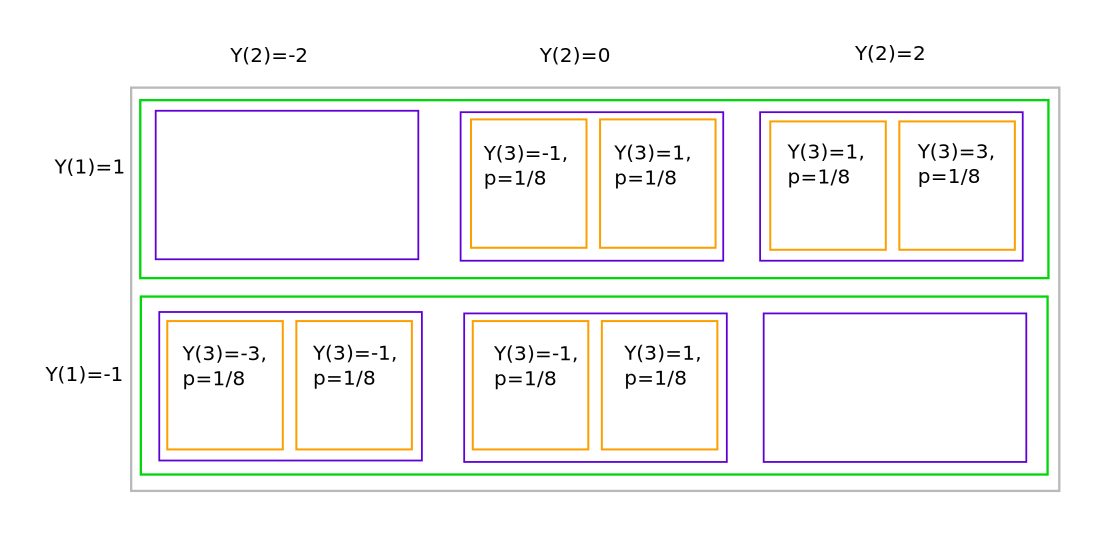
\includegraphics[width=\textwidth]{iter_expect/lie1.pdf}\\
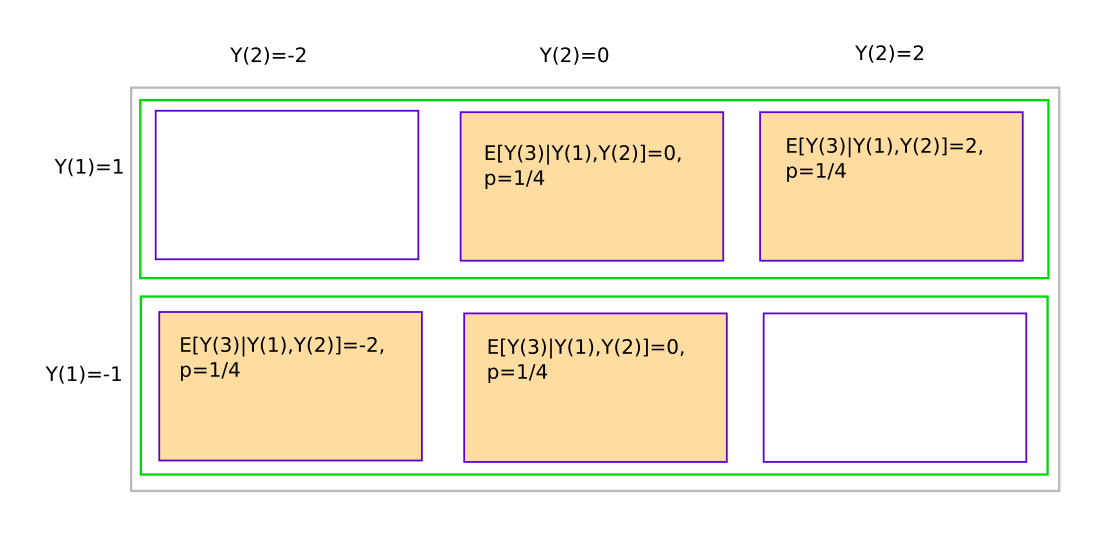
\includegraphics[width=\textwidth]{iter_expect/lie2.pdf}\\
\includegraphics[width=\textwidth]{iter_expect/lie3.pdf}
\caption{Law of iterated expectations, left-hand side}\label{fig:lie-lhs}
\end{figure}

\begin{figure}
\includegraphics[width=\textwidth]{iter_expect/lier1.pdf}\\
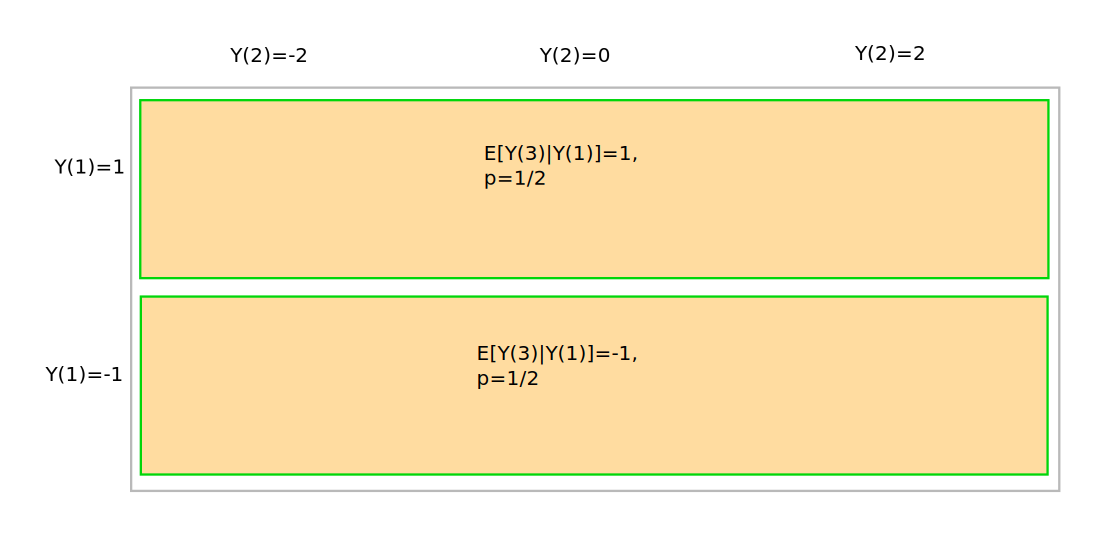
\includegraphics[width=\textwidth]{iter_expect/lier2.pdf}
\caption{Law of iterated expectations, right-hand side}\label{fig:lie-rhs}
\end{figure}

\subsection{Uses}
\subsubsection{Simplifying calculations}
The first use of the law of iterated expectation is to simplify the
calculation of complicated expectations. Examples can be found
in~\cite{ross-probability}. Two results which are useful
in such calculations are as follows.

\begin{prop}\label{prop:conex-funx}
  For any two random variables $X$ and $Y$ and information set $I$, if
  $X$ belongs to the information set $I$ and $h(X)$ is any function of
  $X$ then
  \[E[h(X)Y|I]=h(X)E[Y|I].\]
\end{prop}

\begin{prop}\label{prop:conex-ind}
For any random variable $Y$ and information set $I$, if $Y$ is
  independent of the variables in $I$ then
  \[E[Y|I]=E[Y].\]
\end{prop}

The two results above correspond to two extremes of information
availability. In the first case knowing $I$ gives us full information
about $X$ and therefore functions of $X$ behave like constants and
come out of expectations. In the second case knowing $I$ gives us no
information about $Y$ and therefore the conditional expectation is
the same as the unconditional expectations.

\subsubsection{Gradual Revelation of Information}
The past is known whereas the future is unknown. The future, though,
depends on the past and therefore knowledge about the past is helpful
in predicting the possibilities for the future. As we flow through
time, moments pass from the future, through the present, and into the
past, resulting in an accumulation of knowledge and a change in our
beliefs about the future. A model of macroeconomic dynamics must
incorporate these facts about time and knowledge while not giving up
on the machinery for talking about uncertainty that the
probabilists have developed. 

The way we do this is as follows. We set up our probability model in a
`timeless' way. Thus in Example~\ref{exmp:three-toss-conex} even
though the three tosses happen over time we think of each point in
sample space as specifying the result of all three tosses. For each
point of time~ $t$ an information set~$I_t$ is given which specifies
what an agent knows at that time. This information set breaks up the
sample space into chunks. Thus, for example, if we observe that the
first toss has come up heads we know that the outcome must be one of
$HHH$, $HHT$, $HTH$ or $HTT$. If the first toss had come up tails we
would have known that the outcome must have been one of $THH$, $THT$,
$TTH$ or $TTT$. These are precisely the sets~$C_1$ and~$C_2$ in
Table~\ref{tab:decomp_I1}. Once the results of the second toss comes
in our information set becomes larger and we can narrow down the
possible outcomes and know that we are in one of the sets
$C'_1,\ldots,C'_2$ in Table~\ref{tab:decomp_I2}. Thus the gradual
accumulation of knowledge is modelled by adding an increasing sequence
of information sets to a timeless probability model.\footnote{Our increasing
  sequences of information sets is a special case of the more general
  concept of \newterm{filtrations} used by probabilists to model the
  accumulation of information. See ~\cite{billingsley-prob-measure} for details.} 

To be consistent with this formalisation we require that agents
choices be constant over each chunk created by their information sets.
So if an agent has to make a decision after observing only the first
toss then the agent cannot decide differently for the two outcome
$HHT$ and $HHH$ since at that time the agent does not have enough
information to distinguish between those two outcomes. The agent can
however choose differently for the two outcomes $HHT$ and $THT$ since
knowing the result of the first toss allows her to discriminate
between these two outcomes. This requirement that a random variable
like the agent's choice be constant across each chunk created by an
information set has a formal name---we say that the random variable is
\newterm{measurable} with respect to the information set. By
construction expectation conditional on an information set are always
measurable with respect to that information set.

The notion of measurability allows us to add one more trick useful for
working with conditional expectations. 

\begin{prop}\label{prop:conex-measure}
If $I$ is some information set,
$Y$ is any random variable and $X$ is a random variable measurable
with respect to $I$ then
\[E[XY|I]=XE[Y|I]\]
\end{prop}
This is a generalisation of Proposition~\ref{prop:conex-funx}. If $X$
is measurable with respect to $I$ then it is constant on each chunk
created by $I$ and can therefore can be taken out like a constant
while calculating expectations conditional on $I$.

Agents in macroeconomic models must often forecast the value of future
random variables based on the limited information that they have at an
earlier point of time. The \newterm{rational expectations} assumption,
which is the most common assumption about expectations currently in
macroeconomics, says that this forecast is equal to the conditional
expectation of the future variable based on the agent's current
information set. So if $Y_3^{e,1}$ is an agent's forecast after the
first toss of final
winnings in the game in Example~\ref{exmp:three-toss-conex},
then rational expectation says that
\[Y_3^{e,1}=E[Y_3|I_1].\]
The left-hand side of the above equation is an economic agent's
subjective forecast while the right-hand side is a mathematical
expectation calculated from a probability model. There is no logical
reason why they have to be equal, only an economic assumption that
they are.

Sometimes we have to go further and make forecasts about forecasts.
For example, we may want to forecast after the first toss what we
would think of our final winnings after seeing the second toss.
Applying the assumption of rational expectations to both these
forecasts we get the answer
\[E[E[Y_3|I_2]|I_1].\]
The law of iterated expectations allows us to simplify this to
\[E[Y_3|I_1].\]
Thus the forecast of a forecast is the same as a direct forecast. We
shall take advantage of this simplification again and again in our
future work in macroeconomics. It is one of the reasons that we give
so much importance to the law of iterated expectations.

\section{Martingales}
Let $X_t$ be a sequence of random variables and $I_t$ be a sequence of
information sets such that,
\begin{enumerate}
\item $I_t \subset I_{t+1}$.
\item $X_t$ is measurable with respect to $I_t$.
\item $E[|X_t|]<\infty$.
\item $E[X_{t+1}|I_t]=X_t$.
\end{enumerate}
Then the process $X_t$ is said to be a \newterm{martingale} with
respect to the sequence of information sets $I_t$.

Among the defining characteristics of a martingale given above the
crucial one is the last: $E[X_{t+1}|I_t]=X_t$. This says that
conditional on the information available in period $t$ the random
variable $X_t$ neither grows nor declines in the next period in
expected value terms. In this a martingale process is like the wealth
of a gambler playing a fair game. Some outcomes of the game increase
the gambler's wealth, other outcomes of the game decrease the
gambler's wealth, but since the game is fair the increases and
decreases cancel out on an average.

We can use Proposition~\ref{prop:conex-measure} and the properties of
a martingale to show that
\[E[X_{t+1}-X_t|I_t]=0\]
and therefore if $Y$ is any variable belonging to $I_t$ then
\[E[(X_{t+1}-X_{t})Y]=0\]
so that $X_{t+1}-X_t$ is uncorrelated with $Y$. (Give detailed proofs
of all the claims made in this paragraph so far.) That is, the change
in the value of a martingale process is uncorrelated with all the
information available from the past. Speaking loosely, it is a
`surprise'. And so a martingale is a sum of surprises.

A random walk is an martingale (Prove. Be careful to specify the
sequence of information sets.) This has led some economic literature
to loosely use the term ``random walk'' when discussing martingales.
This usage should be avoided since not all martingales are random walks.

The definition of a martingale tells us about the expectation of a
value of the process in a period conditional on the information in the
exactly preceding period. The following proposition covers the case where
conditioning set and the value is separated by more than one period.

\begin{prop}\label{prop:martingale-mp}
Let $X_t$ be a martingale with respect to the information set sequence
$I_t$. For any $m$ and any $n>0$,
\[E[X_{m+n}|I_m]=X_m.\]
\end{prop}
\begin{proof}
The proof is by mathematical induction on $n$.

For $n=1$ the proof follows directly from the definition of a martingale.

Suppose the lemma is true for $n=k$. Consider the case $n=k+1$.
From the law of
iterated expectations
\[E[X_{m+k+1}|I_m]=E[E[X_{m+k+1}|I_{m+k}]|I_m].\]
The martingale property, applied at time $m+k$ tells us that
\[E[X_{m+k+1}|I_{m+k}]=X_{m+k}.\] 
The assumption that the lemma is true for $n=k$ gives us,
\[E[X_{m+k}|I_m]=X_m.\]
Putting everything together, we have
\[E[X_{m+k+1}|I_m]=E[E[X_{m+k+1}|I_{m+k}]|I_m]=E[X_{m+k}|I_m]=X_m\]
thus establishing the result for $n=k+1$.

Since we have shown that the result is true for $n=1$ and it is true
for $n=k+1$ whenever it is true for $n=k$, it follows from the
principle of mathematical induction that it is true for all $n>0$.
\end{proof}






\chapter{Consumption: Uncertainty}
\section{Euler equation}
In the case of uncertainty in labour incomes, but with certain
interest rates, the Euler equation becomes
\begin{equation}\label{eq:euler-uncertain}
v_t'(c_t)=RE_t[v_{t+1}'(c_{t+1})]
\end{equation}
where $E_t$ denotes the mathematical expectation conditional on information at time~$t$.

\section{Quadratic felicity}
\subsection{Martingale property}
Suppose the felicity (i.e. per-period utility) function is
\[v_t(c_t)=\beta^t(ac_t-0.5c_t^2)\]
where $a$ is some constant.

In this case~\eqref{eq:euler-uncertain} specialises to
\[a-c_t = R\beta(a- E_t c_{t+1})\]
If we further assume that $R=1/\beta$ then
\begin{equation}\label{eq:martingale}
E_t c_{t+1}=c_t
\end{equation}
that is, consumption is a martingale process. 

Since $c_t$ is part of the information set at time $t$, $E_tc_t=c_t$
Therefore, another way to write~\eqref{eq:martingale} is
\[E_t(c_{t+1}-c_t)=0\]
which says that the change in consumption between time $t$ and $t+1$
has no predictable direction based on information at time $t$.

This result is a consequence of the very special
assumptions that we have made. Assuming the same felicity function for
each period (apart from the discount factor $\beta$) and then assuming that
the market rate of discount ($1/R$) equals this subjective discount factor
creates a situation where the consumer has no desire to have a higher
consumption in any particular period of her life either to meet
greater consumption needs or to take advantage of the difference
between market and subjective discount rates. Unconstrained lending
and borrowing mean that the consumer can actually move around her
income across periods so as to achieve this perfect symmetry in her
consumption in the sense of equating expected marginal utility across
periods. But with quadratic felicity expected marginal utility is the
same thing as expected consumption and we have our martingale result.

The long list of assumptions leading up to the martingale result means
that this precise result is not very robust or realistic. Therefore
rather than taking it as a property that is likely to be literally
true, we should understand it as a demonstration of the tendency of
the lending and borrowing behaviour of consumers to delink current
consumption from current income. This tendency will be there as long
as consumers have access to asset markets, though in more realistic
settings it will be overlaid with factors which impart a systematic
pattern to the trajectory of consumption such as a changing pattern of
lifetime consumption needs or differences between the subjective and
market rate of discount.

\subsection{The level of consumption}
The martingale property of consumption only tells us how consumption evolves from one
point to the next, not the \emph{level} of consumption. The level of
consumption would depend on the consumer's resources in terms of her
initial wealth and expected labour income. We now show that this is so
mathematically by deriving an explicit formula for the level of
consumption in the case where consumption is a martingale.

Consider a consumer who stands at period $t$ with wealth $w_t$ and is
planning her future consumption for the periods
$t,t+1,\ldots,T$. Since she cannot leave any bequests or outstanding
debt in period $T$, it must be the case that  her \emph{realized}
stream of consumption ($c_t$) and labour income ($y_t$) must satisfy,
\begin{align}
\sum_{i=t}^T \delta^{i-t} c_i &= \sum_{i=t}^T \delta^{i-t} y_i +
w_t\\
\intertext{Taking expectations as of time $t$,}
\sum_{i=t}^T \delta^{i-t} E_t c_i &= \sum_{i=t}^T \delta^{i-t} E_t y_i +
w_t\\
\intertext{From Proposition~\ref{prop:martingale-mp} on
  page~\pageref{prop:martingale-mp}, $E_tc_i=c_t$ for all
$i>t$. And for $i=t$, $E_tc_t=c_t$ because $c_t$ is known at time
$t$. Hence,}
c_t\sum_{i=t}^T \delta^{i-t}  &= \sum_{i=t}^T \delta^{i-t} E_t y_i +
w_t\label{eq:level-c-pih}\\
c_t&=\frac{1}{\sum_{i=t}^T \delta^{i-t} }\left[ \sum_{i=t}^T \delta^{i-t} E_t y_i +
w_t\right]
\end{align}
Thus the level of consumption in a given period depends on the
expected discounted value of the future stream of labour income over
the entire remaining lifetime as well as initial wealth. This once
again reiterates the idea of the permanent income hypothesis that the
consumption in each period depends not just on income in that period
but on the entire expected path of future income.
\subsection{Increments in consumption}
With an explicit formula for the level of consumption in hand, we can
now try to understand the martingale result better by seeing what it
is exactly that drives changes in consumption.

Rewriting~\eqref{eq:level-c-pih} for period $t+1$ we have,
\begin{align*}
c_{t+1}\sum_{i=t+1}^T \delta^{i-t-1}  &= \sum_{i=t+1}^T \delta^{i-t-1} E_{t+1} y_i +
w_{t+1}\\
\intertext{Substituting $w_{t+1}=(w_t+y_t-c_t)/\delta$,}
c_{t+1}\sum_{i=t+1}^T \delta^{i-t-1}  &= \sum_{i=t+1}^T \delta^{i-t-1} E_{t+1} y_i +
(w_t+y_t-c_t)/\delta\\
\intertext{Multiplying throughout by $\delta$,}
c_{t+1}\sum_{i=t+1}^T \delta^{i-t}  &= \sum_{i=t+1}^T \delta^{i-t} E_{t+1} y_i +
w_t+y_t-c_t\\
\intertext{Subtracting~\eqref{eq:level-c-pih} from this equation}
(c_{t+1}-c_t)\sum_{i=t+1}^T \delta^{i-t}-c_t&=\sum_{i=t+1}^T
\delta^{i-t} (E_{t+1} y_i-E_t y_i) + y_t - E_ty_t-c_t\\
\intertext{But $E_ty_t=y_t$ since income at time $t$ is known at that
time,}
(c_{t+1}-c_t)\sum_{i=t+1}^T \delta^{i-t}&=\sum_{i=t+1}^T
\delta^{i-t} (E_{t+1} y_i-E_t y_i)\\
c_{t+1}-c_t&=\frac{1}{\sum_{i=t+1}^T \delta^{i-t}}\left[\sum_{i=t+1}^T
\delta^{i-t} (E_{t+1} y_i-E_t y_i)\right]\\
\end{align*}
We can divide both the numerator and denominator by $\delta$ to have
the factor multiplying the first term in the sums equal to
one.\footnote{This is a purely aesthetic change and does not change
  any results.} This gives us our final formula,
\begin{equation}\label{eq:increment-cons}
c_{t+1}-c_t=\frac{1}{\sum_{i=t+1}^T \delta^{i-t-1}}\left[\sum_{i=t+1}^T
\delta^{i-t-1} (E_{t+1} y_i-E_t y_i)\right]
\end{equation}
What the formula above says is that changes in consumption are
a result of \emph{revisions} in expectations of future income based on
the difference in information at time $t$ and $t+1$. Therefore
changes in income that were predictable at time $t$ do not contribute
to the change in consumption between time $t$ and $t+1$. This is
consistent with our assumption that consumption is a martingale but
goes further by predicting the actual size of the consumption change
rather than just asserting that the expected value of this change
would be zero.

\subsection{Specific income processes}
In general the difference in expectations which occur on the right
of~\eqref{eq:increment-cons} depends on all the information which
becomes available to the consumer between time $t$ and $t+1$. One
special case which we now consider is when the only source of new
information is the realisation of the labour income $y_{t+1}$. What
revision this new information causes in the expectation of future
labour income depends on how labour income in different periods are related.

As an example consider the labour income process given by the
following stochastic difference equation,
\begin{equation}\label{eq:def-ar1}
y_{t+1}-\mu=\rho(y_t-\mu)+\epsilon_{t+1}
\end{equation}
where $\epsilon_t$ is a white-noise process, $\mu$ and $\rho$ are
constants and $0 < \rho <1$. This is a special case of what is known
as a first-order autoregressive process (sometimes denoted as a AR(1)
process). The coefficient $\rho$ measures how persistent the
deviations in $y$ from its long-run average $\mu$ are.

Writing~\eqref{eq:def-ar1} for the period $t+2$ we have,
\[y_{t+2}-\mu=\rho(y_{t+1}-\mu)+\epsilon_{t+2}\]
Substituting~\eqref{eq:def-ar1},
\[y_{t+2}-\mu=\rho^2(y_t-\mu)+\rho\epsilon_{t+1}+\epsilon_{t+2}\]
Carrying out successive substitutions like this, we find for any
$i>t$
\[y_i-\mu = \rho^{i-t}(y_t-\mu)+\sum_{j=t+1}^i \rho^{i-j} \epsilon_j\]
Taking expectations conditional on the information at time $t$,
\[E_t(y_i-\mu) = \rho^{i-t}(y_t-\mu)+\sum_{j=t+1}^i \rho^{i-j}
E_t\epsilon_j\]
Here we have used the fact that $y_t$ is known at time $t$. We
further note that since $\epsilon_t$ is IID, $\epsilon_j$ is
independent of all information at time $t$ when $j>t$ and we can
replace $E_t \epsilon_j$ by $E \epsilon_j$ which is $0$ by the
definition of white noise. Hence we conclude,
\begin{equation}\label{eq:ar-cond-t}
E_t(y_i-\mu) = \rho^{i-t}(y_t-\mu) \qquad \text{for $i \geq t$}
\end{equation}
(We have established this above for $i>t$ and it is trivially true for
$i=t$.)

Using $t+1$ in the place of $t$,
\begin{equation}\label{eq:ar-cond-t1}
E_{t+1}(y_i-\mu) = \rho^{i-t-1}(y_{t+1}-\mu) \qquad \text{for $i \geq t+1$}
\end{equation}

For $i\geq t+1$ both~\eqref{eq:ar-cond-t} and~\eqref{eq:ar-cond-t1}
hold. Subtracting the former from the latter we have,
\begin{align*}
E_{t+1} y_i - E_t y_i &=
\rho^{i-t-1}(y_{t+1}-\mu)-\rho^{i-t}(y_t-\mu)\\
\intertext{Using~\eqref{eq:def-ar1},}
&=\rho^{i-t-1}[\rho(y_t-\mu)+\epsilon_{t+1}]-\rho^{i-t}(y_t-\mu)\\
&=\rho^{i-t-1}\epsilon_{t+1}
\end{align*}

Substituting this in~\eqref{eq:increment-cons} we get,
\[c_{t+1}-c_t=\left[\frac{\sum_{i=t+1}^T(\delta\rho)^{i-t-1}}
{\sum_{i=t+1}^T \delta^{i-t-1}}\right]\epsilon_{t+1}\]
So we see that for a given innovation in consumption,
$\epsilon_{t+1}$, the increment in consumption is higher the higher is
the degree of persistence $\rho$ in the income process.

In empirical applications of the model we can estimate $\rho$ (or its
analogues for more complex income processes) from
data on consumers' incomes  and then check if changes in consumption
satisfy the forumla above. This yields a sharper test of our theory
compared to just checking if consumption is a martingale.

\chapter{Overlapping Generations}
The Ramsey model is at least in two ways a well-behaved model. First,
the market equilibrium in the model is always Pareto optimal. Second,
the dynamics of the model is very simple. Regardless of what capital
stock we start the model with, both the capital/labour ratio and
consumption/labour ratio move monotonically\footnote{that is, without
  changing their direction of movement} towards their steady-state
values.

This simplicity of the Ramsey model is deceptive. Even within the
Ramsey framework, very complex dynamics is possible if we consider
multisector models rather than the single-good model that we have
studied. However, equilibria are Pareto efficient in all Ramsey
models, so this complex dynamics is still efficient.

This is not the case in the overlapping generations models that we
consider in this chapter. These models can demonstrate both complex
dynamics and Pareto suboptimal equilibria. These models are completely
orthodox methodologically: all agents in these economies are
optimisers and have perfect foresight and all markets are competitive
and in equilibrium at all times. Therefore their behaviour is even
more surprising and causes us to question our understanding of the
behaviour of even idealised competitive market economies. 

An overlapping generations economy is an infinite-horizon economy in
which the agents can be grouped into different `generations' such that
the following properties hold.
\begin{enumerate}
\item At each point of time members of different generations coexist.
\item There are generations whose lifetime is not the same
as the lifetime of the entire economy.
\end{enumerate}

The above definition tries to capture the essence of the many
different varieties of overlapping generations economies that have
been studied in the literature. However, in this chapter we shall
limit ourselves to very simple examples. We will find instances of
counter-intuitive behaviour in even these simple cases.

\section{Pure exchange: Incomplete Participation}
Our first example is that of a pure exchange economy, i.e.\ an economy
without production. Time is discrete and doubly infinite: there is an
infinite past as well as an infinite future. 

Agents have a two-period lifetime. At the beginning of each period a
new generation of agents is born, which dies at the end of the next
period. Following convention, we refer to the agents in the first
period of their lives as `young' and in the second period of their
lives as `old' respectively.

All agents in the same generation are identical and each generation
has the same number of agents. Because of these assumptions we can
replace each generation by a single representative agent.

There is a single physical good in the economy which is not storable.
Each agent is endowed with some quantity of this good in each of the
periods of their lives.

Even though there is only one physical commodity, agents care not only
about how much of this commodity they have but also when they have it.
Therefore in economic terms we need to tag the quantities of the
commodities with dates on which those quantities would be available.
Thus, even with a single physical commodity there is a separate
economic commodity corresponding to the delivery of this physical
commodity on a particular date. Since our model has infinite number of
periods we therefore have an infinity of economic commodities in our
model. We call these economic commodities `dated-commodities' to
indicate that along with a physical description each commodity is also
marked with a delivery date.

In this section we assume that in every period markets open to allow
trading in all dated-commodities. Only those agents who live in a
particular period can participate in that period's market. Neither the
unborn nor the dead can trade. It is because of this last assumption
that the model of this section is called a model of limited participation.

To keep things simple we assume that every generation is alike in
terms of having the same pattern of endowments and the same
preferences over consumption streams. Note that this does not mean
that the two periods of an agent's lifetime are alike. It is possible
that the agents want to consume more when they are old. Or perhaps
agents are richer when they are young. All we are assuming is that if
one generation is richer when it is young then so are all generations
and so on. This assumption of stationarity means that every period
looks alike in our model. But in each period some agents are young and
some are old and this is enough to generate interesting phenomena
since we allow endowments and preferences to be age-dependent.

\subsection{Notation}
We will denote agent-specific variables by two subscripts: the first
to indicate whether the variables pertains to the young~($1$) or old
($2$) and the second to indicate the date to which the variable
pertains. So an agent born in period~$t$, who lives in the periods~$t$
and $t+1$ will have the consumption stream $(c_{1,t},c_{2,t+1})$ since
the consumer will be young in period~$t$ and old in period~$t+1$. On
the other hand the total consumption in period~$t$ will be
$c_{1,t}+c_{2,t}$ since we need to add up the consumption of the young
and the old, belonging to different generations, who live in period
$t$.

Our assumption of stationarity makes the notation simpler for
endowments and utility functions. All generations have the same
endowment stream $(\omega_1,\omega_2)$ and utility function
$U(c_{1,t},c_{2,t+1})$.

\subsection{Equilibrium}
The way we have set up the model there is no opportunity to trade.
Because there is only one good there are no trades within a period
since there is no point buying and selling the same good. Therefore
all trade must be across time, or in simpler language, the only
possible trades involve borrowing and lending. Since each generation
is homogeneous there cannot be any trade between members of the same
generation. If one member of a generation wants to borrow then so do
all members of that generation and vice versa. Finally, and most
importantly, there can be no trade between generations because two
agents of different generations meet only in one period. Today's old
cannot trade with today's young since the former will not be around
tomorrow to repay a loan they receive or collect on a loan they give.
Today's young cannot trade with tomorrow's young since the latter have
not been born yet.

Thus in the way we have set up the model there can be no trade and the
only possible equilibrium is the autarky equilibrium in which each
agent consumes her endowment.

In general equilibrium theory for economies with a finite number of
goods and agents all competitive equilibrium are necessary Pareto
optimal. This result is known as the ``First Fundamental Theorem of
Welfare Economics''.\footnote{See \cite[16.C]{mascolell}. The
  additional technical assumption of local non-satiation of
  preferences is required. This is satisfied in all our examples.} The
following examples shows that this theorem does not necessarily hold
for overlapping generations model.

\begin{exmp}\label{exmp:olg-np-single}
Consider the economy as described above with the utility function
for the initial old given by
\[u(c_{2,0})=\ln(1+c_{2,0})\]
and utility function for later generations given by
\[u(c_{1,t},c_{2,t+1})=\ln(1+c_{1,t})+\ln(1+c_{2,t+1}).\]

Suppose endowments are $\omega_1=1,\omega_2=0$.

The autarkic equilibrium involves everyone consuming their endowments,
i.e.
\[c_{1,t}=1, c_{2,t}=0\]
The utility of the initial old under this equilibrium is
\[u(c_{2,0})=\ln (1+0)=0\]
and the utility of all later generations is
\[u(c_{1,t},c_{2,t+1})=\ln(1+1)+\ln(1+0)=\ln 2.\]

It turns out that this allocation is not Pareto optimal. Consider the
alternative allocation
\[\hat c_{1,t}=\hat c_{2,t}=1/2\]
We first check that this allocation is feasible given the economy's
resources
\[\hat c_{1,t}+\hat c_{2,t}=\omega_1+\omega_2=1\]

The utility of the initial old under the hat allocation is higher
\[u(\hat c_{2,0})=\ln (1+1/2) = \ln 3/2 >0\]

The utility of all other generations under the hat allocation is also
higher
\[u(\hat c_{1,t},\hat c_{2,t+1})=\ln (1+1/2)+\ln(1+1/2)=\ln (3/2)^2 >
\ln 2.\]

Thus the hat allocation is a feasible allocation that makes all agents
better off than the competitive allocation. Thus it is a Pareto
improvement over the competitive allocation and its existence shows
that the competitive allocation is not Pareto optimal.

\qed
\end{exmp}

\begin{exmp}\label{exmp:olg-np-double}
Consider an economy with the same structure as before but in which
time is doubly infinite, i.e.\ time neither has a beginning nor an
end. Because there is no initial period there is no initial old
generation to consider. All generations are alike. Each generation has
the utility function
\[u(c_{1,t},c_{2,t+1})=\ln(1+c_{1,t})+\ln(1+c_{2,t+1}).\]
and the endowment
\[\omega_1=0, \omega_2=1.\]

Once again, because any two generations meet only in a single period
no trade is possible and the equilibrium allocation is the autarkic
one
\[c_{1,t}=0, c_{2,t}=1\]

The alternative allocation
\[\hat c_{1,t}=1/2, \hat c_{2,t}=1/2\]
is feasible and we can check that it makes every generation strictly
better off. So the autarkic equilibrium is once again not Pareto
optimal.

\qed
\end{exmp}

The failure of the First Fundamental Theorem in these examples is
since this theorem has very few explicit assumptions and a
straightforward proof and therefore would be expected to hold quite
generally. What is going wrong?

The infinity of time certainly has a role to play. In
Example~\ref{exmp:olg-np-single} the Pareto improvement comes about
because each generation gives up half a unit of the consumption goods
to its elders during its youth and in return receives half a unit of
the consumption good from its juniors in its own old age. If there had
been an end of time then the last generation would not have had any
juniors to compensate them and would have been worse off. Then the new
allocation would no longer be a Pareto improvement. In
Example~\ref{exmp:olg-np-double} the direction of transfers is the
opposite and hence there would be no Pareto improvement if there had
been a beginning of time.

However, the infinity of time cannot by itself explain the failure of
the First Fundamental Theorem. The Ramsey model provides a
counterexample of a type of economy which also has infinite time
but where the First Fundamental Theorem always holds.

One property which differentiates overlapping generations models
from both finite equilibrium models and the Ramsey model is the
property of limited participation. Only agents who are alive on a
certain date are allowed to buy and sell commodities deliverable on
that date. The unborn and the dead are excluded from markets. While
this is certainly reasonable from an economic point of view, can it be
this exclusion which is responsible for the possibility of competitive
equilibria not being Pareto optimal in this model?

\section{Pure Exchange Economies: Complete Participation}
To see whether it is the incompleteness of market participation which
leads to non-Pareto optimal equilibria, we modify the overlapping
generations by allowing all agents to trade in all dated commodities
and looking for equilibrium prices. We might imagine a marketplace
that stands outside of time, in which souls can trade for delivery of
commodities at any point of time. We look for prices at which the
demands and supplies of the souls of different generations match. We
show by an example that even when completing the markets in this
manner there still can be equilibria which are not Pareto optimal.

\begin{exmp}\label{exmp:olg-complete}
We continue with the economy of Example~\ref{exmp:olg-np-double} in
which time is doubly infinite, preferences are given by
\[u(c_{1,t},c_{2,t+1})=\ln(1+c_{1,t})+\ln(1+c_{2,t+1}).\]
and endowments are
\[\omega_1=0,\, \omega_2=1.\]

Suppose that the price of the good in period~$t$ is~$p_t$. Then the
consumer born in time~$t$ solves the problem
\[\max_{c_{1,t},c_{2,t+1}} \ln(1+c_{1,t})+\ln(1+c_{2,t+1})\]
subject to
\[p_t(\omega_1-c_{1,t})=p_{t+1}(c_{2,t+1}-\omega_2)\]

Assuming an interior solution the solution to this optimisation
problem is\footnote{Exercise: derive this.}

\begin{equation}\label{eq:olg-complete-demand}
c_{1,t}=\frac{2(p_{t+1}/p_t)-1}{2},\quad
c_{2,t+1}=\frac{p_t}{2p_{t+1}}
\end{equation}

Equilibrium requires
\begin{equation}\label{eq:olg-complete-equil}
c_{1,t}+c_{2,t}=\omega_1+\omega_2=1,\qquad \text{for all $t$}
\end{equation}

There are many sequence of prices which satisfy the above equilibrium
conditions. Here are two interesting ones.

First, the sequence $(\ldots,4,2,1,\nicefrac{1}{2},\nicefrac{1}{4},\ldots)$. That is
$p_t=1/2^t$ for all~$t$. With these prices we see
from~\eqref{eq:olg-complete-demand} that $c_{1,t}=0, c_{2,t+1}=1$ for
all~$t$ which satisfies~\eqref{eq:olg-complete-equil}. This is an
equilibrium in which every agent consumes their endowment---an
allocation which we have shown to be Pareto inferior
earlier.\footnote{We derived our demand
  functions~\eqref{eq:olg-complete-demand} assuming an interior
  solution to the consumer's maximisation problem. On the other hand,
  the allocation in this case lies on the boundary of the consumption
  set since $c_{1,t}=0$. Why is this not a problem?}

Second, consider the prices $(\ldots,1,1,1,\ldots)$. That is $p_t=1$
for all~$t$. For these prices $c_{1,t}=1/2, c_{2,t+1}=1/2$ which again
satisfies~\eqref{eq:olg-complete-equil}. This allocation is an Pareto
improvement on the previous allocation and we show in the appendix to
this chapter that it is in fact Pareto optimal, that is there is no
possibility of a further Pareto improvement from this allocation.

\qed
\end{exmp}

Example~\ref{exmp:olg-complete} shows that Pareto suboptimal
equilibria can persist in an overlapping generations economy even when
we assume that all agents can participate in all markets. Thus it is
not incomplete participation which is to blame for the Pareto
suboptimality. Rather, it is the combination of an infinite horizon
and an infinity of agents who do not live forever which is to blame
for the failure of the First Welfare Theorem. 

\section{Money}
Overlapping generations models have also been used as a tool for
studying monetary economies. Modern fiat money---unlike money based on
precious metals---is intrinsically worthless. It is neither useful as
an object of consumption nor is it useful as a factor of production.
It is demanded only in the expectation that it will be accepted in
exchange for useful goods. But those who accept money must in turn expect
that it will be accepted by others when they try to spend it. This
dependence of the value of money on the general belief in its
acceptability is captured well by overlapping generations models.

Consider an economy with singly-infinite time. The initial old have a
utility function given by
\[u_0(c_{2,0})\]
and other generations have an utility function
\[u(c_{1,t},c_{2,t+1}).\]
Endowments in the two periods are~$\omega_1$ and~$\omega_2$ respectively.

Only living people can trade. As we discussed earlier, with this
assumption the only equilibrium in this model is an autarkic one.
Example~\ref{exmp:olg-np-single} shows that this autarkic equilibrium
might not be Pareto optimal.

Now suppose we endow the initial old with $M$ units of useless but
durable green pieces of paper that we call `money'. Assume that just
like goods this money can also be traded by agents alive at each date.
Let $p_t$ be the price of the consumption good in terms of money at
time $t$.

The decision problem of the initial old is simple. Since they have
only one period to live and money is useless they sell the money for
whatever it is worth in terms of consumption goods. So we have
\begin{equation}\label{eq:olg-money-initial}
c_{2,0}=M/p_0
\end{equation}

The later generations now have the choice of selling some goods in
their youth and acquiring money. Since money is durable they can carry
it over to their old age and spend it for consumption goods then. If
we denote by $M^d_t$ the amount of money demanded in their youth by
the generation born in period~$t$ then the optimisation problem for
that generation is
\[\max_{c_{1,t},c_{2,t+1},M^d_t} u(c_{1,t},c_{2,t+1})\]
subject to
\begin{align*}
p_t(\omega_1-c_{1,t})&=M^d_t\\
p_{t+1}(c_{2,t+1}-\omega_2)&=M^d_t\\
M^d_t&\ge 0
\end{align*}

If we define real money demand by $m^d_t=M^d_t/p_t$ and the relative
increase in prices by $\pi_{t+1}=p_{t+1}/p_t$ then the above
optimization problem can be rewritten as
\[\max_{c_{1,t},c_{2,t+1},m^d_t} u(c_{1,t},c_{2,t+1})\]
subject to
\begin{align*}
\omega_1-c_{1,t}&=m^d_t\\
c_{2,t+1}-\omega_2&=m^d_t/\pi_{t+1}\\
m^d_t&\ge 0
\end{align*}

This form of the optimisation problem makes it clear that the real
money stock demanded by a young agent equals that agent's real savings
and $1/\pi_{t+1}$ is the returns that the agent earns on her savings.

The solution of the optimisation problem gives us $m^d_t$, $c_{1,t}$
and $c_{2,t+1}$ as functions of $\pi_{t+1}$. In particular we define
\[m^d_t = L(1/\pi_{t+1})\]

Equilibrium in the money market requires
\begin{equation}\label{eq:olg-money-money}
L(1/\pi_{t+1}) = M/p_t
\end{equation}
Equilibrium in the goods market requires
\begin{equation}\label{eq:olg-money-goods}
c_{1,t}+c_{2,t} = \omega_1+\omega_2
\end{equation}

From Walras' law we know that if one of these equilibrium conditions
is satisfied then the other will be satisfied automatically.

For periods $t>0$ we can use the consumer's budget constraint to
rewrite~\eqref{eq:olg-money-goods} as follows
\begin{equation}\label{eq:olg-money-diffeq}
\begin{split}
c_{1,t}+c_{2,t} &= \omega_1+\omega_2\\
c_{2,t}-\omega_2 &= \omega_1-c_{1,t}\\
m^d_{t-1}/\pi_t & = m^d_t\\
L(1/\pi_t)\frac{1}{\pi_t} &= L(1/\pi_{t+1})
\end{split}
\end{equation}

Using~\eqref{eq:olg-money-money} for $t=0$
and~\eqref{eq:olg-money-diffeq} for $t>0$ and remembering that Walras'
law allows us to use just one equilibrium condition per period we have
the equilibrium conditions
\begin{align}
L(1/\pi_1)&=M/p_0\\
L(1/\pi_t)\frac{1}{\pi_t} &= L(1/\pi_{t+1}), \qquad t>0
\end{align}

For simplicity let us look at steady state equilibria where $\pi_t$
and hence $c_{1,t}$ and $c_{2,t}$ are constants. Then the equilibrium
conditions become,
\begin{align}
\label{eq:olg-money-steady0} L(1/\pi)&=M/p_0\\
\label{eq:olg-money-steadyt} L(1/\pi)(1/\pi) &= L(1/\pi)
\end{align}

There are two solutions to these equations. The first is a value of
$\pi=\pi^*$ where 
\[L(\pi^*)=0.\]
There is always such a $\pi^*$ since if we take the relative price
ratio between consumption in the two periods to be equal to the
consumer's marginal rate of substitution at the endowment point then
the consumer is happy consuming her endowment and does not want to
hold any money.

If $L(\pi^*)=0$ then~\eqref{eq:olg-money-steady0} cannot strictly be
satisfied if $M>0$. However, loosely speaking we can say that this
equation is satisfied with $p_0=\infty$. An infinite price of good in
terms of money means that it is impossible to buy even the smallest
amount of goods with any amount of money however large. Money is thus
valueless in this equilibrium and everyone continues to consume their
endowment.\footnote{If you are uncomfortable with infinity as a price,
  you can get rid of it as follows. Rather than choosing money as the
  numeriare choose an abstract numeriare in terms of which $\mu_t$ is
  the price of money and $\lambda_t$ is the price of goods in 
  period~$t$. Arguing as above then you will find an equilibrium with
  $\mu_t=0$ for all $t$. Our $p_t=\lambda_t/\mu_t$ and hence it turns
  out to be infinite in this equilibrium.}

The other steady-state solution is the one with $\pi=1$. In this
case~\eqref{eq:olg-money-steadyt} is automatically satisfied
and~\eqref{eq:olg-money-steady0} gives us
\[p_0 = M/L(1)\]
If $L(1)=0$ then this once again gives us a equilibrium with
$p_0=\infty$ where money is not valued. But if $L(1)>1$ then we have
an equilibrium in which money has a constant value in the steady
state. Thus even if money is useless it is possible to have an
equilibrium with valued money in an overlapping generations model.


\section*{Appendix}
\begin{prop}
In the overlapping generations model with utility function
\[u(c_{1,t},c_{2,t+1})=\ln(1+c_{1,t})+\ln(1+c_{2,t+1}),\]
stationary endowments $\omega_1=1, \omega_2=0$ and doubly-infinite
time, the stationary allocation $c_{1,t}=1/2,c_{2,t}=1/2$ is Pareto
optimal.
\end{prop}

\subsection*{The main idea}
If the allocation mentioned in the proposition is not Pareto optimal then
there must be another allocation which is a Pareto improvement, i.e.\
which makes everyone at least as well off and at least one agent
strictly better off. Let us denote this allocation by $(\hat
c_{1,t},\hat c_{2,t})$. 

Since any leftover output can be given to some agent to make them
better off without making anyone worse off, we assume we have already
done so, so that,
\begin{equation}\label{eq:olg-hat-feas}
\hat c_{1,t}+\hat c_{2,t} = \omega_1+\omega_2 =1
\end{equation}

If the allocation with the hats is different from
$(1/2,1/2)$ there must be some~$t$ for which $\hat c_{1,t} \ne 1/2$ or
$\hat c_{2,t} \ne 1/2$. From~\eqref{eq:olg-hat-feas} it then follows
that for that~$t$ either $\hat c_{1,t}>1/2$ or $\hat c_{2,t}>1/2$. (Why?)

Assume that $\hat c_{2,t}>1/2$ for some $t$. 

(The argument remains basically unchanged when $\hat c_{1,t}>1/2$ if
time is doubly infinite. All that we have to do is to look at periods
before~$t$ rather than at periods after~$t$ as we do below. A little
more change is required if time has a beginning. Try to think through
both these cases once you have studied the case where $\hat
c_{2,t}>1/2$.)

If $\hat c_{2,t}>1/2$ then from~\eqref{eq:olg-hat-feas} it must be the
case that $\hat c_{1,t}<1/2$. That is, the young born in period~$t$
consume less in their youth under the hat allocation than they did in
the initial allocation. But if the hat allocation is to be a Pareto
improvement then these period-$t$ young have to be at least as well
off under the hat allocation as under the original allocation. This
can happen only if they consume more in their old age under the hat
allocation than under the original allocation. So, it must be that
$\hat c_{2,t+1}>1/2$.

Let 
\begin{align*}
\delta_t &= 1/2-\hat c_{1,t}\\
\phi_t &= \hat c_{2,t+1}-1/2
\end{align*}

We are looking at the case where $\delta_t>0$ and we have argued in the
last paragraph that $\phi_t>0$. In fact we can do better than that.
Here's how. Consider the possibility that $\phi_t=\delta_t$. Then
\begin{align*}
u(\hat c_{1,t},\hat c_{2,t+1})
&=u(1/2-\delta_t,1/2+\phi_t)\\
&=u(1/2-\delta_t,1/2+\delta_t)\\
&=\ln(1+1/2-\delta_t)+\ln(1+1/2+\delta_t)\\
&=\ln[(3/2-\delta_t)(3/2+\delta_t)]\\
&=\ln[9/4-\delta_t^2]\\
&< \ln(9/4)=u(c_{1,t},c_{2,t+1})
\end{align*}

Thus increasing consumption in old age by the same amount as
consumption is reduced in youth will make the generation-$t$ agent
strictly worse off than she was under the original $(1/2,1/2)$
allocation. Therefore if the hat allocation is to keep the consumer at
least as well off as before it must be the case that
\begin{equation}\label{eq:olg-phi-delta}
\phi_t>\delta_t
\end{equation}

But where is this extra consumption going to come from? It can only
come by reducing the consumption of the young in period~$t+1$. Since
\begin{align*}
\hat c_{1,t+1}+\hat c_{2,t+1}&=1=1/2+1/2\\
\intertext{It must be the case that,}
1/2-\hat c_{1,t+1} &= \hat c_{2,t+1}-1/2
\end{align*}
If we define $\delta_{t+1}=1/2-\hat c_{1,t+1}$ the above shows that
\[\delta_{t+1}=\phi_t>\delta_t>0\]

Defining $\phi_{t+1}=\hat c_{2,t+2}-1/2$ and applying the argument
that we applied to generation~$t$ to generation~$(t+1)$ we find that
\[\delta_{t+2}=\phi_{t+1}>\delta_{t+1}>0\]

Continuing to repeat this argument we get the chain of inequalities
\begin{equation}\label{eq:delta-chain}
\delta_t < \delta_{t+1} < \delta_{t+2} < \cdots
\end{equation}

The above chain of inequalities shows that $\delta_k$ increases with
$k$. But there is an upper bound on $\delta_k$. Since 
\[\delta_k = 1/2-\hat c_{1,k}\] 
and $\hat c_{1,k} \ge 0$ it must be the case that 
\begin{equation}\label{eq:bound-delta}
\delta_k \le 1/2
\end{equation}

If we could use~\eqref{eq:delta-chain} to argue that $\delta_k$ grows
without bounds then that would contradict~\eqref{eq:bound-delta} and
we would have succeeded in proving that it is not possible to
construct a Pareto improvement over the original allocation
$(1/2,1/2)$.

Unfortunately this is not the case. Equation~\eqref{eq:delta-chain}
does not imply unbounded growth of $\delta_k$. A sequence like
\[0.4,0.44,0.444,0.4444,\ldots\]
can satisfy both~\eqref{eq:delta-chain} and~\eqref{eq:bound-delta}. So
in order to be successful in our proof we have to find a way to
strengthen~\eqref{eq:delta-chain}.

\subsection*{A stronger inequality}
As before we define
\begin{align*}
\delta_k&=1/2-\hat c_{1,k}>0\\
\phi_k&=\hat c_{2,k+1}-1/2>0
\end{align*}

Also as before feasibility requires
\begin{equation}\label{eq:olg-feas}
\phi_k=\delta_{k+1}
\end{equation}

For the hat allocation to be a Pareto improvement it is necessary that
\begin{align*}
u(\hat c_{1,k},\hat c_{2,k+1}) &\ge u(c_{1,k},c_{2,k+1})\\
u(1/2-\delta_k,1/2+\phi_k) &\ge u(1/2,1/2)\\
\ln [(3/2-\delta_k)(3/2+\phi_k)] &\ge \ln (9/4)\\
\frac{9}{4} + \frac{3}{2}\phi_k - \frac{3}{2}\delta_k -\delta_k\phi_k
&\ge \frac{9}{4}\\
\frac{\phi_k}{\delta_k} &\ge \frac{1}{1-2\delta_k/3}
\end{align*}

Now we know from~\eqref{eq:delta-chain} that $\delta_t \le \delta_k$
for $k \ge t$. Applying this to the denominator of the above
expression and remembering that $\delta_t \le 1/2$
from~\eqref{eq:bound-delta} we have
\begin{equation*}
\frac{\phi_k}{\delta_k} 
\ge \frac{1}{1-2\delta_t/3} 
\ge \frac{1}{1-2\cdot(1/2)/3} = 3/2
\end{equation*}

But $\phi_k=\delta_{k+1}$ so we have
\begin{equation}\label{eq:olg-delta-strong}
\frac{\delta_{k+1}}{\delta_k} \ge 3/2
\end{equation}

This says that in each period~$\delta$ grows at least~1.5 times. As a
result it will grow unboundedly starting from any nonzero value.
Formally, by starting from time~$t$ and chaining
together~\eqref{eq:olg-delta-strong} together $j$~times we have
\[\delta_{t+j} \ge (3/2)^j \delta_t\]
Provided $\delta_t>0$ the right-hand side becomes larger than $1/2$
for large enough~$j$ and hence contradicts~\eqref{eq:bound-delta},
thus proving that no Pareto improvement over our original allocation
is possible.

\subsection*{Generalisation}
The inequalities~\eqref{eq:delta-chain}
and~\eqref{eq:olg-delta-strong} were derived using a particular
functional form of the utility function and a particular initial
allocation. But the style of reasoning we have used above can be
generalised to provide a criteria for Pareto optimality applicable to
arbitrary utility functions and arbitrary allocations. See
Proposition~5.6 of~\cite{balasko1980overlapping}.












\backmatter
\bibliographystyle{alpha} \bibliography{macro}

\end{document}
